%&preformat-disser
\RequirePackage[l2tabu,orthodox]{nag} % Раскомментировав, можно в логе получать рекомендации относительно правильного использования пакетов и предупреждения об устаревших и нерекомендуемых пакетах
% Формат А4, 14pt (ГОСТ Р 7.0.11-2011, 5.3.6)
\documentclass[a4paper,14pt,oneside,openany]{memoir}

%%%%%%%%%%%%%%%%%%%%%%%%%%%%%%%%%%%%%%%%%%%%%%%%%%%%%%%%%%%%%%%%%%%%%%%%%%%%%%%%
%%%% Файл упрощённых настроек шаблона, общих для диссертации и автореферата %%%%
%%%%%%%%%%%%%%%%%%%%%%%%%%%%%%%%%%%%%%%%%%%%%%%%%%%%%%%%%%%%%%%%%%%%%%%%%%%%%%%%

%%% Режим черновика %%%
\makeatletter
\@ifundefined{c@draft}{
  \newcounter{draft}
  \setcounter{draft}{0}  % 0 --- чистовик (максимальное соблюдение ГОСТ)
                         % 1 --- черновик (отклонения от ГОСТ, но быстрая
                         %       сборка итоговых PDF)
}{}
\makeatother

%%% Пометки в тексте %%%
\makeatletter
\@ifundefined{c@showmarkup}{
  \newcounter{showmarkup}
  \setcounter{showmarkup}{0}  % 0 --- скрыть пометки
                              % 1 --- показывать пометки
}{}
\makeatother

%%% Диссертация на английском %%%
\makeatletter
\@ifundefined{c@englishthesis}{
  \newcounter{englishthesis}
  \setcounter{englishthesis}{1}  % 0 --- диссертация на русском
                                 % 1 --- диссертация на английском; влияет 
                                 %       на подписи к рисункам и прочее
}{}
\makeatother

%%% Использование в pdflatex шрифтов не по-умолчанию %%%
\makeatletter
\@ifundefined{c@usealtfont}{
  \newcounter{usealtfont}
  \setcounter{usealtfont}{1}    % 0 --- шрифты на базе Computer Modern
                                % 1 --- использовать пакет pscyr, при его
                                %       наличии
                                % 2 --- использовать пакет XCharter, при наличии
                                %       подходящей версии
}{}
\makeatother

%%% Использование в xelatex и lualatex семейств шрифтов %%%
\makeatletter
\@ifundefined{c@fontfamily}{
  \newcounter{fontfamily}
  \setcounter{fontfamily}{1}  % 0 --- CMU семейство. Используется как fallback;
                              % 1 --- Шрифты от MS (Times New Roman и компания)
                              % 2 --- Семейство Liberation
}{}
\makeatother

%%% Библиография %%%
\makeatletter
\@ifundefined{c@bibliosel}{
  \newcounter{bibliosel}
  \setcounter{bibliosel}{1}   % 0 --- встроенная реализация с загрузкой файла
                              %       через движок bibtex8;
                              % 1 --- реализация пакетом biblatex через движок
                              %       biber
}{}
\makeatother

%%% Вывод типов ссылок в библиографии %%%
\makeatletter
\@ifundefined{c@mediadisplay}{
  \newcounter{mediadisplay}
  \setcounter{mediadisplay}{1}   % 0 --- не делать ничего; надписи [Текст] и
                                 %       [Эл. ресурс] будут выводиться только в ссылках с
                                 %       заполненным полем `media`;
                                 % 1 --- автоматически добавлять надпись [Текст] к ссылкам с
                                 %       незаполненным полем `media`; таким образом, у всех
                                 %       источников будет указан тип, что соответствует
                                 %       требованиям ГОСТ
                                 % 2 --- автоматически удалять надписи [Текст], [Эл. Ресурс] и др.;
                                 %       не соответствует ГОСТ
                                 % 3 --- автоматически удалять надпись [Текст];
                                 %       не соответствует ГОСТ
                                 % 4 --- автоматически удалять надпись [Эл. Ресурс];
                                 %       не соответствует ГОСТ
}{}
\makeatother

%%% Предкомпиляция tikz рисунков для ускорения работы %%%
\makeatletter
\@ifundefined{c@imgprecompile}{
  \newcounter{imgprecompile}
  \setcounter{imgprecompile}{1}   % 0 --- без предкомпиляции;
                                  % 1 --- пользоваться предварительно
                                  %       скомпилированными pdf вместо генерации
                                  %       заново из tikz
}{}
\makeatother
            % общие настройки шаблона
%%% Проверка используемого TeX-движка %%%
\newif\ifxetexorluatex   % определяем новый условный оператор (http://tex.stackexchange.com/a/47579)
\ifxetex
    \xetexorluatextrue
\else
    \ifluatex
        \xetexorluatextrue
    \else
        \xetexorluatexfalse
    \fi
\fi

\newif\ifsynopsis           % Условие, проверяющее, что документ --- автореферат

\usepackage{etoolbox}[2015/08/02]   % Для продвинутой проверки разных условий
\providebool{presentation}

\usepackage{comment}    % Позволяет убирать блоки текста (добавляет
                        % окружение comment и команду \excludecomment)

%%% Поля и разметка страницы %%%
\usepackage{pdflscape}  % Для включения альбомных страниц
\usepackage{geometry}   % Для последующего задания полей

%%% Математические пакеты %%%
\usepackage{amsthm,amsmath,amscd}   % Математические дополнения от AMS
\usepackage{amsfonts,amssymb}       % Математические дополнения от AMS
\usepackage{mathtools}              % Добавляет окружение multlined
\usepackage{xfrac}                  % Красивые дроби
\usepackage[
    locale = DE,
    list-separator       = {;\,},
    list-final-separator = {;\,},
    list-pair-separator  = {;\,},
    list-units           = single,
    range-units          = single,
    range-phrase={\text{\ensuremath{-}}},
    % quotient-mode        = fraction, % красивые дроби могут не соответствовать ГОСТ
    fraction-function    = \sfrac,
    separate-uncertainty,
    ]{siunitx}[=v2]                 % Размерности SI
\sisetup{inter-unit-product = \ensuremath{{}\cdot{}}}


% Кириллица в нумерации subequations
% Для правильной работы требуется выполнение сразу после загрузки пакетов
\ifnumequal{\value{englishthesis}}{0}{
    \patchcmd{\subequations}{\def\theequation{\theparentequation\alph{equation}}}
    {\def\theequation{\theparentequation\asbuk{equation}}}
    {\typeout{subequations patched}}{\typeout{subequations not patched}}
}{}
% \patchcmd{\subequations}{\def\theequation{\theparentequation\alph{equation}}}
% {\def\theequation{\theparentequation\asbuk{equation}}}
% {\typeout{subequations patched}}{\typeout{subequations not patched}}

%%%% Установки для размера шрифта 14 pt %%%%
%% Формирование переменных и констант для сравнения (один раз для всех подключаемых файлов)%%
%% должно располагаться до вызова пакета fontspec или polyglossia, потому что они сбивают его работу
\newlength{\curtextsize}
\newlength{\bigtextsize}
\setlength{\bigtextsize}{13.9pt}

\makeatletter
%\show\f@size    % неплохо для отслеживания, но вызывает стопорение процесса,
                 % если документ компилируется без команды  -interaction=nonstopmode
\setlength{\curtextsize}{\f@size pt}
\makeatother

%%% Кодировки и шрифты %%%
\ifxetexorluatex
    \ifpresentation
        \providecommand*\autodot{} % quick fix for polyglossia 1.50
    \fi
    \PassOptionsToPackage{no-math}{fontspec}    % https://tex.stackexchange.com/a/26295/104425
    \usepackage{polyglossia}[2014/05/21]        % Поддержка многоязычности
                                        % (fontspec подгружается автоматически)
\else
   %%% Решение проблемы копирования текста в буфер кракозябрами
    \ifnumequal{\value{usealtfont}}{0}{}{
        \input glyphtounicode.tex
        \input glyphtounicode-cmr.tex %from pdfx package
        \pdfgentounicode=1
    }
    \usepackage{cmap}   % Улучшенный поиск русских слов в полученном pdf-файле
    \ifnumequal{\value{usealtfont}}{2}{}{
        \defaulthyphenchar=127  % Если стоит до fontenc, то переносы
                                % не впишутся в выделяемый текст при
                                % копировании его в буфер обмена
    }
    \usepackage{textcomp}
    \usepackage[T1,T2A]{fontenc}                    % Поддержка русских букв
    \ifnumequal{\value{usealtfont}}{1}{% Используется pscyr, при наличии
        \IfFileExists{pscyr.sty}{\usepackage{pscyr}}{}  % Подключение pscyr
    }{}
    \usepackage[utf8]{inputenc}[2014/04/30]         % Кодировка utf8
    \ifnumequal{\value{englishthesis}}{0}{
        \usepackage[english, russian]{babel}[2014/03/24]% Языки: русский, английский
    }{
        \usepackage[english]{babel}[2014/03/24]% Языки: английский
    }



    \makeatletter\AtBeginDocument{\let\@elt\relax}\makeatother % babel 3.40 fix
    \ifnumequal{\value{usealtfont}}{2}{
        % http://dxdy.ru/post1238763.html#p1238763
        \usepackage[scaled=0.914]{XCharter}[2017/12/19] % Подключение русифицированных шрифтов XCharter
        \usepackage[charter, vvarbb, scaled=1.048]{newtxmath}[2017/12/14]
        \ifpresentation
        \else
            \setDisplayskipStretch{-0.078}
        \fi
    }{}
\fi

%%% Оформление абзацев %%%
\ifpresentation
\else
    \indentafterchapter     % Красная строка после заголовков типа chapter
    \usepackage{indentfirst}
\fi

%%% Цвета %%%
\ifpresentation
\else
    \usepackage[dvipsnames, table, hyperref]{xcolor} % Совместимо с tikz
\fi

%%% Таблицы %%%
\usepackage{longtable,ltcaption} % Длинные таблицы
\usepackage{multirow,makecell}   % Улучшенное форматирование таблиц
\usepackage{tabu, tabulary}      % таблицы с автоматически подбирающейся
                                 % шириной столбцов (tabu обязательно
                                 % до hyperref вызывать)
\makeatletter
%https://github.com/tabu-issues-for-future-maintainer/tabu/issues/26
\@ifpackagelater{longtable}{2020/02/07}{
\def\tabuendlongtrial{%
    \LT@echunk  \global\setbox\LT@gbox \hbox{\unhbox\LT@gbox}\kern\wd\LT@gbox
                \LT@get@widths
}%
}{}
\makeatother

\usepackage{threeparttable}      % автоматический подгон ширины подписи таблицы

%%% Общее форматирование
\usepackage{soulutf8}% Поддержка переносоустойчивых подчёркиваний и зачёркиваний
\usepackage{icomma}  % Запятая в десятичных дробях

%%% Оптимизация расстановки переносов и длины последней строки абзаца
\IfFileExists{impnattypo.sty}{% проверка установленности пакета impnattypo
    \ifluatex
        \ifnumequal{\value{draft}}{1}{% Черновик
            \usepackage[hyphenation, lastparline, nosingleletter, homeoarchy,
            rivers, draft]{impnattypo}
        }{% Чистовик
            \usepackage[hyphenation, lastparline, nosingleletter]{impnattypo}
        }
    \else
        \usepackage[hyphenation, lastparline]{impnattypo}
    \fi
}{}

%% Векторная графика

\usepackage{tikz}                   % Продвинутый пакет векторной графики
\usetikzlibrary{chains}             % Для примера tikz рисунка
\usetikzlibrary{shapes.geometric}   % Для примера tikz рисунка
\usetikzlibrary{shapes.symbols}     % Для примера tikz рисунка
\usetikzlibrary{arrows}             % Для примера tikz рисунка

%%% Гиперссылки %%%
\ifxetexorluatex
    \let\CYRDZE\relax
\fi
\usepackage[draft]{hyperref}[2012/11/06]

%%% Изображения %%%
\usepackage{graphicx}[2014/04/25]   % Подключаем пакет работы с графикой
\usepackage{caption}                % Подписи рисунков и таблиц
\usepackage{subcaption}             % Подписи подрисунков и подтаблиц
\usepackage{pdfpages}               % Добавление внешних pdf файлов

%%% Счётчики %%%
\usepackage{aliascnt}
\usepackage[figure,table]{totalcount}   % Счётчик рисунков и таблиц
\usepackage{totcount}   % Пакет создания счётчиков на основе последнего номера
                        % подсчитываемого элемента (может требовать дважды
                        % компилировать документ)
\usepackage{totpages}   % Счётчик страниц, совместимый с hyperref (ссылается
                        % на номер последней страницы). Желательно ставить
                        % последним пакетом в преамбуле

%%% Продвинутое управление групповыми ссылками (пока только формулами) %%%
\ifpresentation
\else
    \ifnumequal{\value{englishthesis}}{0}{
        \usepackage[russian]{cleveref} % cleveref имеет сложности со считыванием
    % языка из babel. Такое решение русификации вывода выбрано вместо
    % определения в documentclass из опасности что-то лишнее передать во все
    % остальные пакеты, включая библиографию.
    }{
        \usepackage{cleveref}
    }
    % Добавление возможности использования пробелов в \labelcref
    % https://tex.stackexchange.com/a/340502/104425
    \usepackage{kvsetkeys}
    \makeatletter
    \let\org@@cref\@cref
    \renewcommand*{\@cref}[2]{%
        \edef\process@me{%
            \noexpand\org@@cref{#1}{\zap@space#2 \@empty}%
        }\process@me
    }
    \makeatother
\fi

\usepackage{placeins} % для \FloatBarrier

\ifnumequal{\value{draft}}{1}{% Черновик
    \usepackage[firstpage]{draftwatermark}
    \SetWatermarkText{DRAFT}
    \SetWatermarkFontSize{14pt}
    \SetWatermarkScale{15}
    \SetWatermarkAngle{45}
}{}

%%% Цитата, не приводимая в автореферате:
% возможно, актуальна только для biblatex
%\newcommand{\citeinsynopsis}[1]{\ifsynopsis\else ~\cite{#1} \fi}

% если текущий процесс запущен библиотекой tikz-external, то прекомпиляция должна быть включена
\ifdefined\tikzexternalrealjob
    \setcounter{imgprecompile}{1}
\fi

\ifnumequal{\value{imgprecompile}}{1}{% Только если у нас включена предкомпиляция
    \usetikzlibrary{external}   % подключение возможности предкомпиляции
    \tikzexternalize[prefix=images/cache/,optimize command away=\includepdf] % activate! % здесь можно указать отдельную папку для скомпилированных файлов
    \ifxetex
        \tikzset{external/up to date check={diff}}
    \fi
}{}


\usepackage{physics}
\usepackage{bbm}
\usepackage{qcircuit}
\usepackage{tabularx}
\usepackage[export]{adjustbox}
\usepackage{oplotsymbl}
% \usepackage{generic}
% \usepackage{cite}
% \usepackage{amsmath,amssymb,amsfonts}
% \usepackage{graphicx}
% \usepackage{textcomp}
% \pagestyle{empty}

%sampling packages
% % \usepackage{cite}
% \usepackage{amsmath,amssymb,amsfonts}
% \usepackage{graphicx}
% \usepackage{textcomp}
% \usepackage{lipsum}

% % The preceding line is only needed to identify funding in the first footnote. If that is unneeded, please comment it out.
% \usepackage{textcomp}
% %\usepackage{xcolor}
% \usepackage{verbatim}

% \usepackage{algorithm}
% \usepackage{algorithmic}
% \usepackage{algorithmicx,algpseudocode}
\usepackage[ruled]{algorithm2e}
\usepackage{pgfplots}
\pgfplotsset{compat=1.16} 
\usepackage{lscape}

\usepackage{rotating} 


% \usepackage{hyperref}

% %\usepackage{amsthm}
% \usepackage{amssymb}
% \usepackage{amsmath}
% \usepackage{multirow}
% %\usepackage{xcolor}
% \usepackage{tikz}
% \usetikzlibrary{calc,shapes.geometric,arrows,positioning,intersections}
% %\usepackage{pagecolor}
% \usetikzlibrary{decorations, decorations.text,backgrounds}
% % \usepackage{color}         % Пакеты общие для диссертации и автореферата
\synopsisfalse                      % Этот документ --- не автореферат
%%% Прикладные пакеты %%%
%\usepackage{calc}               % Пакет для расчётов параметров, например длины

%%% Для добавления Стр. над номерами страниц в оглавлении
%%% http://tex.stackexchange.com/a/306950
\usepackage{afterpage}

%%% Списки %%%
\usepackage{enumitem}

%%% Абзацный отступ у первого абзаца после заголовков
\usepackage{indentfirst}

%%% Оформление списка обозначений
\usepackage[intoc]{nomencl}
\makenomenclature
\setlength{\nomitemsep}{-.8\parsep}
    % Пакеты для диссертации
\input{Dissertation/userpackages}   % Пакеты для специфических пользовательских задач

%%%%%%%%%%%%%%%%%%%%%%%%%%%%%%%%%%%%%%%%%%%%%%%%%%%%%%
%%%% Файл упрощённых настроек шаблона диссертации %%%%
%%%%%%%%%%%%%%%%%%%%%%%%%%%%%%%%%%%%%%%%%%%%%%%%%%%%%%

%%% Инициализирование переменных, не трогать!  %%%
\newcounter{intvl}
\newcounter{otstup}
\newcounter{contnumeq}
\newcounter{contnumfig}
\newcounter{contnumtab}
\newcounter{pgnum}
\newcounter{chapstyle}
\newcounter{headingdelim}
\newcounter{headingalign}
\newcounter{headingsize}
%%%%%%%%%%%%%%%%%%%%%%%%%%%%%%%%%%%%%%%%%%%%%%%%%%%%%%

%%% Область упрощённого управления оформлением %%%

%% Интервал между заголовками и между заголовком и текстом %%
% Заголовки отделяют от текста сверху и снизу
% тремя интервалами (ГОСТ Р 7.0.11-2011, 5.3.5)
\setcounter{intvl}{3}               % Коэффициент кратности к размеру шрифта

%% Отступы у заголовков в тексте %%
\setcounter{otstup}{0}              % 0 --- без отступа; 1 --- абзацный отступ

%% Нумерация формул, таблиц и рисунков %%
% Нумерация формул
\setcounter{contnumeq}{0}   % 0 --- пораздельно (во введении подряд,
                            %       без номера раздела);
                            % 1 --- сквозная нумерация по всей диссертации
% Нумерация рисунков
\setcounter{contnumfig}{0}  % 0 --- пораздельно (во введении подряд,
                            %       без номера раздела);
                            % 1 --- сквозная нумерация по всей диссертации
% Нумерация таблиц
\setcounter{contnumtab}{1}  % 0 --- пораздельно (во введении подряд,
                            %       без номера раздела);
                            % 1 --- сквозная нумерация по всей диссертации

%% Оглавление %%
\setcounter{pgnum}{1}       % 0 --- номера страниц никак не обозначены;
                            % 1 --- Стр. над номерами страниц (дважды
                            %       компилировать после изменения настройки)
\settocdepth{subsection}    % до какого уровня подразделов выносить в оглавление
\setsecnumdepth{subsubsection} % до какого уровня нумеровать подразделы


%% Текст и форматирование заголовков %%
\setcounter{chapstyle}{1}     % 0 --- разделы только под номером;
                              % 1 --- разделы с названием "Глава" перед номером
\setcounter{headingdelim}{1}  % 0 --- номер отделен пропуском в 1em или \quad;
                              % 1 --- номера разделов и приложений отделены
                              %       точкой с пробелом, подразделы пропуском
                              %       без точки;
                              % 2 --- номера разделов, подразделов и приложений
                              %       отделены точкой с пробелом.

%% Выравнивание заголовков в тексте %%
\setcounter{headingalign}{0}  % 0 --- по центру;
                              % 1 --- по левому краю

%% Размеры заголовков в тексте %%
\setcounter{headingsize}{0}   % 0 --- по ГОСТ, все всегда 14 пт;
                              % 1 --- пропорционально изменяющийся размер
                              %       в зависимости от базового шрифта

%% Подпись таблиц %%

% Смещение строк подписи после первой строки
\newcommand{\tabindent}{0cm}

% Тип форматирования заголовка таблицы:
% plain --- название и текст в одной строке
% split --- название и текст в разных строках
\newcommand{\tabformat}{plain}

%%% Настройки форматирования таблицы `plain`

% Выравнивание по центру подписи, состоящей из одной строки:
% true  --- выравнивать
% false --- не выравнивать
\newcommand{\tabsinglecenter}{false}

% Выравнивание подписи таблиц:
% justified   --- выравнивать как обычный текст («по ширине»)
% centering   --- выравнивать по центру
% centerlast  --- выравнивать по центру только последнюю строку
% centerfirst --- выравнивать по центру только первую строку (не рекомендуется)
% raggedleft  --- выравнивать по правому краю
% raggedright --- выравнивать по левому краю
\newcommand{\tabjust}{justified}

% Разделитель записи «Таблица #» и названия таблицы
\newcommand{\tablabelsep}{~\cyrdash\ }

%%% Настройки форматирования таблицы `split`

% Положение названия таблицы:
% \centering   --- выравнивать по центру
% \raggedleft  --- выравнивать по правому краю
% \raggedright --- выравнивать по левому краю
\newcommand{\splitformatlabel}{\raggedleft}

% Положение текста подписи:
% \centering   --- выравнивать по центру
% \raggedleft  --- выравнивать по правому краю
% \raggedright --- выравнивать по левому краю
\newcommand{\splitformattext}{\raggedright}

%% Подпись рисунков %%
%Разделитель записи «Рисунок #» и названия рисунка
\newcommand{\figlabelsep}{~\cyrdash\ }  % (ГОСТ 2.105, 4.3.1)
                                        % "--- здесь не работает

%%% Цвета гиперссылок %%%
% Latex color definitions: http://latexcolor.com/
% \definecolor{linkcolor}{rgb}{0.9,0,0}
% \definecolor{citecolor}{rgb}{0,0.6,0}
% \definecolor{urlcolor}{rgb}{0,0,1}
\definecolor{linkcolor}{rgb}{0,0,0} %black
\definecolor{citecolor}{rgb}{0,0,0} %black
\definecolor{urlcolor}{rgb}{0,0,0} %black
      % Упрощённые настройки шаблона

\input{common/newnames}         % Новые переменные, для всего проекта

%%% Основные сведения %%%
\newcommand{\thesisAuthorLastName}{Салников}
\newcommand{\thesisAuthorOtherNames}{Михаил}
\newcommand{\thesisAuthorInitials}{М.}
\newcommand{\thesisAuthorLastNameEn}{Salnikov}
\newcommand{\thesisAuthorOtherNamesEn}{Mikhail}
\newcommand{\thesisAuthorInitialsEn}{M.}

\newcommand{\thesisAuthor}             % Диссертация, ФИО автора
{%
    \texorpdfstring{% \texorpdfstring takes two arguments and uses the first for (La)TeX and the second for pdf
        \thesisAuthorLastName~\thesisAuthorOtherNames% так будет отображаться на титульном листе или в тексте, где будет использоваться переменная
    }{%
        \thesisAuthorLastName, \thesisAuthorOtherNames% эта запись для свойств pdf-файла. В таком виде, если pdf будет обработан программами для сбора библиографических сведений, будет правильно представлена фамилия.
    }
}
\newcommand{\thesisAuthorEn}             % Диссертация, ФИО автора
{%
    \texorpdfstring{% \texorpdfstring takes two arguments and uses the first for (La)TeX and the second for pdf
        \thesisAuthorLastNameEn~\thesisAuthorOtherNamesEn% так будет отображаться на титульном листе или в тексте, где будет использоваться переменная
    }{%
        \thesisAuthorLastNameEn, \thesisAuthorOtherNamesEn% эта запись для свойств pdf-файла. В таком виде, если pdf будет обработан программами для сбора библиографических сведений, будет правильно представлена фамилия.
    }
}

\newcommand{\thesisAuthorShort}        % Диссертация, ФИО автора инициалами
{\thesisAuthorInitials~\thesisAuthorLastName}
\newcommand{\thesisAuthorShortEn}        % Диссертация, ФИО автора инициалами
{\thesisAuthorInitialsEn~\thesisAuthorLastNameEn}

%\newcommand{\thesisUdk}                % Диссертация, УДК
%{\fixme{xxx.xxx}}
\newcommand{\thesisTitle}              % Диссертация, название
{LLM hallucination}
\newcommand{\thesisTitleEn}              % Диссертация, название
{LLM hallucination}
\newcommand{\thesisSpecialtyNumber}    % Диссертация, специальность, номер
{1.2.2}%05.13.18
\newcommand{\thesisSpecialtyTitle}     % Диссертация, специальность, название (название взято с сайта ВАК для примера)
{Математическое моделирование, численные методы и комплексы программ}
\newcommand{\thesisSpecialtyTitleEn}     % Диссертация, специальность, название (название взято с сайта ВАК для примера)
{Mathematical modeling, numerical methods and program complexes}
%% \newcommand{\thesisSpecialtyTwoNumber} % Диссертация, вторая специальность, номер
%% {\fixme{XX.XX.XX}}
%% \newcommand{\thesisSpecialtyTwoTitle}  % Диссертация, вторая специальность, название
%% {\fixme{Теория и~методика физического воспитания, спортивной тренировки,
%% оздоровительной и~адаптивной физической культуры}}
\newcommand{\thesisDegree}             % Диссертация, ученая степень
{кандидата физико-математических наук}
\newcommand{\thesisDegreeEn}             % Диссертация, ученая степень
{Doctor of Philosophy in Physics and Mathematics}
\newcommand{\thesisDegreeShort}        % Диссертация, ученая степень, краткая запись
{канд.~физ.-мат.~наук}
\newcommand{\thesisDegreeShortEn}        % Диссертация, ученая степень, краткая запись
{PhD.~in Phys.-Math.}
\newcommand{\thesisCity}               % Диссертация, город написания диссертации
{Москва}
\newcommand{\thesisCityEn}               % Диссертация, город написания диссертации
{Moscow}
\newcommand{\thesisYear}               % Диссертация, год написания диссертации
{2024}
\newcommand{\thesisOrganization}       % Диссертация, организация
{Автономная некоммерческая образовательная организация высшего образования <<Сколковский институт науки и технологий>>}
\newcommand{\thesisOrganizationNonTitle}       % Диссертация, организация
{Автономная некоммерческая образовательная организация высшего образования <<Сколковский институт науки и технологий>>}
\newcommand{\thesisOrganizationEn}       % Диссертация, организация
{Autonomous Non-Profit Organization for Higher Education\\<<Skolkovo Institute of Science and Technology>>}
\newcommand{\thesisOrganizationEnNonTitle}       % Диссертация, организация
{Autonomous Non-Profit Organization for Higher Education <<Skolkovo Institute of Science and Technology>>}
\newcommand{\thesisOrganizationShort}  % Диссертация, краткое название организации для доклада
{Сколтех}
\newcommand{\thesisOrganizationShortEn}  % Диссертация, краткое название организации для доклада
{Skoltech}

\newcommand{\thesisInOrganization}     % Диссертация, организация в предложном падеже: Работа выполнена в ...
{Автономной некоммерческой образовательной организации высшего профессионального образования <<Сколковский институт науки и технологий>>}

%% \newcommand{\supervisorDead}{}           % Рисовать рамку вокруг фамилии
\newcommand{\supervisorFio}              % Научный руководитель, ФИО
{Елена Николаевна Грязина}
\newcommand{\supervisorRegalia}          % Научный руководитель, регалии
{доктор компьютерных наук, кандидат физико-математических наук}
\newcommand{\supervisorFioShort}         % Научный руководитель, ФИО
{Е.\,Н.~Грязина}
\newcommand{\supervisorRegaliaShort}     % Научный руководитель, регалии
{д.~к.~н, к.ф.-м.н.}

\newcommand{\supervisorFioEn}              % Научный руководитель, ФИО
{Elena Nikolaevna Gryazina}
\newcommand{\supervisorRegaliaEn}          % Научный руководитель, регалии
{Doctor of Computer Sciences, Candidate of Physical and Mathematical Sciences}
\newcommand{\supervisorFioShortEn}         % Научный руководитель, ФИО
{\fixme{E.\,N.~Gryazina}}
\newcommand{\supervisorRegaliaShortEn}     % Научный руководитель, регалии
{\fixme{D.Sc., c.p.-m.s}}

%% \newcommand{\supervisorTwoDead}{}        % Рисовать рамку вокруг фамилии
%% \newcommand{\supervisorTwoFio}           % Второй научный руководитель, ФИО
%% {\fixme{Фамилия Имя Отчество}}
%% \newcommand{\supervisorTwoRegalia}       % Второй научный руководитель, регалии
%% {\fixme{уч. степень, уч. звание}}
%% \newcommand{\supervisorTwoFioShort}      % Второй научный руководитель, ФИО
%% {\fixme{И.\,О.~Фамилия}}
%% \newcommand{\supervisorTwoRegaliaShort}  % Второй научный руководитель, регалии
%% {\fixme{уч.~ст.,~уч.~зв.}}

\newcommand{\opponentOneFio}           % Оппонент 1, ФИО
{\fixme{Фамилия Имя Отчество}}
\newcommand{\opponentOneRegalia}       % Оппонент 1, регалии
{\fixme{доктор физико-математических наук, профессор}}
\newcommand{\opponentOneJobPlace}      % Оппонент 1, место работы
{\fixme{Не очень длинное название для места работы}}
\newcommand{\opponentOneJobPost}       % Оппонент 1, должность
{\fixme{старший научный сотрудник}}

\newcommand{\opponentTwoFio}           % Оппонент 2, ФИО
{\fixme{Фамилия Имя Отчество}}
\newcommand{\opponentTwoRegalia}       % Оппонент 2, регалии
{\fixme{кандидат физико-математических наук}}
\newcommand{\opponentTwoJobPlace}      % Оппонент 2, место работы
{\fixme{Основное место работы c длинным длинным длинным длинным названием}}
\newcommand{\opponentTwoJobPost}       % Оппонент 2, должность
{\fixme{старший научный сотрудник}}

%% \newcommand{\opponentThreeFio}         % Оппонент 3, ФИО
%% {\fixme{Фамилия Имя Отчество}}
%% \newcommand{\opponentThreeRegalia}     % Оппонент 3, регалии
%% {\fixme{кандидат физико-математических наук}}
%% \newcommand{\opponentThreeJobPlace}    % Оппонент 3, место работы
%% {\fixme{Основное место работы c длинным длинным длинным длинным названием}}
%% \newcommand{\opponentThreeJobPost}     % Оппонент 3, должность
%% {\fixme{старший научный сотрудник}}

\newcommand{\opponentOneFioEn}           % Оппонент 1, ФИО
{\fixme{Name name name}}
\newcommand{\opponentOneRegaliaEn}       % Оппонент 1, регалии
{\fixme{Doctor of physcial and mathematical sciences, Professor}}
\newcommand{\opponentOneJobPlaceEn}      % Оппонент 1, место работы
{\fixme{Somewhat long job place name}}
\newcommand{\opponentOneJobPostEn}       % Оппонент 1, должность
{\fixme{Senior research scientist}}

\newcommand{\opponentTwoFioEn}           % Оппонент 2, ФИО
{\fixme{Name name name}}
\newcommand{\opponentTwoRegaliaEn}       % Оппонент 2, регалии
{\fixme{Doctor of physcial and mathematical sciences}}
\newcommand{\opponentTwoJobPlaceEn}      % Оппонент 2, место работы
{\fixme{Main job place with a long long long long long long, reeeeally long title}}
\newcommand{\opponentTwoJobPostEn}       % Оппонент 2, должность
{\fixme{Senior research scientist}}

\newcommand{\leadingOrganizationTitle} % Ведущая организация, дополнительные строки. Удалить, чтобы не отображать в автореферате
{...}
\newcommand{\leadingOrganizationTitleEn} % Ведущая организация, дополнительные строки. Удалить, чтобы не отображать в автореферате
{...}

\newcommand{\defenseDate}              % Защита, дата
{«5» февраля 2025 года в 12 часов 30 минут}
\newcommand{\defenseDateEn}              % Защита, дата
{February 5, 2025, at 12:30 p.m.}
\newcommand{\defenseCouncilNumber}     % Защита, номер диссертационного совета
{1.2.2.2.}
\newcommand{\defenseCouncilNumberEn}     % Защита, номер диссертационного совета
{1.2.2.2.}
\newcommand{\defenseCouncilTitle}      % Защита, учреждение диссертационного совета
{\fixme{Название учреждения}}
\newcommand{\defenseCouncilTitleEn}      % Защита, учреждение диссертационного совета
{\fixme{Defence council title}}
\newcommand{\defenseCouncilAddress}    % Защита, адрес учреждение диссертационного совета
{Территория Инновационного Центра «Сколково», Большой бульвар д.30, стр.1, Москва 121205}
\newcommand{\defenseCouncilAddressEn}    % Защита, адрес учреждение диссертационного совета
{The territory of the Skolkovo Innovation Center, Bolshoy Boulevard, 30, p.1, Moscow 121205}
\newcommand{\defenseCouncilPhone}      % Телефон для справок
{\fixme{+7~(0000)~00-00-00}}

\newcommand{\defenseSecretaryFio}      % Секретарь диссертационного совета, ФИО
{Копелевич Григорий Александрович}
\newcommand{\defenseSecretaryRegalia}  % Секретарь диссертационного совета, регалии
{кандидат физико-математических наук}            % Для сокращений есть ГОСТы, например: ГОСТ Р 7.0.12-2011 + http://base.garant.ru/179724/#block_30000

\newcommand{\defenseSecretaryFioEn}      % Секретарь диссертационного совета, ФИО
{Kopelevich Grigoriy Aleksandrovich}
\newcommand{\defenseSecretaryRegaliaEn}  % Секретарь диссертационного совета, регалии
{Candidate of Physical and Mathematical Sciences}    

\newcommand{\synopsisLibrary}          % Автореферат, название библиотеки
{Сколтеха и на сайте организации https://dissovet.skoltech.ru}
\newcommand{\synopsisDate}             % Автореферат, дата рассылки
{<<\rule[-0.1cm]{0.75cm}{0.15mm}>>\rule[-0.1cm]{3cm}{0.15mm} \the\year~г}

\newcommand{\synopsisLibraryEn}          % Автореферат, название библиотеки
{library of Skoltech or on the website https://dissovet.skoltech.ru}
\newcommand{\synopsisDateEn}             % Автореферат, дата рассылки
{<<\rule[-0.1cm]{0.75cm}{0.15mm}>>\rule[-0.1cm]{3cm}{0.15mm}, \the\year}

% To avoid conflict with beamer class use \providecommand
\providecommand{\keywords}%            % Ключевые слова для метаданных PDF диссертации и автореферата
{}
             % Основные сведения
\input{common/fonts}            % Определение шрифтов (частичное)
\ifnumequal{\value{englishthesis}}{1}{
    \input{common/styles_en}           % Стили общие для диссертации и автореферата
}{
    \input{common/styles}           % Стили общие для диссертации и автореферата
}

%%% Переопределение именований, если иначе не сработает %%%
%\gappto\captionsrussian{
%    \renewcommand{\chaptername}{Глава}
%    \renewcommand{\appendixname}{Приложение} % (ГОСТ Р 7.0.11-2011, 5.7)
%}

%%% Изображения %%%
\graphicspath{{images/}{Dissertation/images/}}         % Пути к изображениям

%%% Интервалы %%%
%% По ГОСТ Р 7.0.11-2011, пункту 5.3.6 требуется полуторный интервал
%% Реализация средствами класса (на основе setspace) ближе к типографской классике.
%% И правит сразу и в таблицах (если со звёздочкой)
%\DoubleSpacing*     % Двойной интервал
\OnehalfSpacing*    % Полуторный интервал
%\setSpacing{1.42}   % Полуторный интервал, подобный Ворду (возможно, стоит включать вместе с предыдущей строкой)

%%% Макет страницы %%%
% Выставляем значения полей (ГОСТ 7.0.11-2011, 5.3.7)
\geometry{a4paper, top=2cm, bottom=2cm, left=2.5cm, right=1cm, nofoot, nomarginpar} %, heightrounded, showframe
\setlength{\topskip}{0pt}   %размер дополнительного верхнего поля
\setlength{\footskip}{12.3pt} % снимет warning, согласно https://tex.stackexchange.com/a/334346

%%% Выравнивание и переносы %%%
%% http://tex.stackexchange.com/questions/241343/what-is-the-meaning-of-fussy-sloppy-emergencystretch-tolerance-hbadness
%% http://www.latex-community.org/forum/viewtopic.php?p=70342#p70342
\tolerance 1414
\hbadness 1414
\emergencystretch 1.5em % В случае проблем регулировать в первую очередь
% Глобально отключаем переносы слов
\hyphenpenalty=10000
\exhyphenpenalty=10000
\righthyphenmin=62
\hfuzz 0.3pt
\vfuzz \hfuzz
%\raggedbottom
%\sloppy                 % Избавляемся от переполнений
\clubpenalty=10000      % Запрещаем разрыв страницы после первой строки абзаца
\widowpenalty=10000     % Запрещаем разрыв страницы после последней строки абзаца
\brokenpenalty=4991     % Ограничение на разрыв страницы, если строка заканчивается переносом

%%% Блок управления параметрами для выравнивания заголовков в тексте %%%
\newlength{\otstuplen}
\setlength{\otstuplen}{\theotstup\parindent}
\ifnumequal{\value{headingalign}}{0}{% выравнивание заголовков в тексте
    \newcommand{\hdngalign}{\centering}                % по центру
    \newcommand{\hdngaligni}{}% по центру
    \setlength{\otstuplen}{0pt}
}{%
    \newcommand{\hdngalign}{}                 % по левому краю
    \newcommand{\hdngaligni}{\hspace{\otstuplen}}      % по левому краю
} % В обоих случаях вроде бы без переноса, как и надо (ГОСТ Р 7.0.11-2011, 5.3.5)

%%% Оглавление %%%
\renewcommand{\cftchapterdotsep}{\cftdotsep}                % отбивка точками до номера страницы начала главы/раздела

%% Переносить слова в заголовке не допускается (ГОСТ Р 7.0.11-2011, 5.3.5). Заголовки в оглавлении должны точно повторять заголовки в тексте (ГОСТ Р 7.0.11-2011, 5.2.3). Прямого указания на запрет переносов в оглавлении нет, но по той же логике невнесения искажений в смысл, лучше в оглавлении не переносить:
\setrmarg{2.55em plus1fil}                             %To have the (sectional) titles in the ToC, etc., typeset ragged right with no hyphenation
\renewcommand{\cftchapterpagefont}{\normalfont}        % нежирные номера страниц у глав в оглавлении
\renewcommand{\cftchapterleader}{\cftdotfill{\cftchapterdotsep}}% нежирные точки до номеров страниц у глав в оглавлении
%\renewcommand{\cftchapterfont}{}                       % нежирные названия глав в оглавлении

\ifnumgreater{\value{headingdelim}}{0}{%
    \renewcommand\cftchapteraftersnum{.\space}       % добавляет точку с пробелом после номера раздела в оглавлении
}{}
\ifnumgreater{\value{headingdelim}}{1}{%
    \renewcommand\cftsectionaftersnum{.\space}       % добавляет точку с пробелом после номера подраздела в оглавлении
    \renewcommand\cftsubsectionaftersnum{.\space}    % добавляет точку с пробелом после номера подподраздела в оглавлении
    \renewcommand\cftsubsubsectionaftersnum{.\space} % добавляет точку с пробелом после номера подподподраздела в оглавлении
    \AfterEndPreamble{% без этого polyglossia сама всё переопределяет
        \setsecnumformat{\csname the#1\endcsname.\space}
    }
}{%
    \AfterEndPreamble{% без этого polyglossia сама всё переопределяет
        \setsecnumformat{\csname the#1\endcsname\quad}
    }
}

\renewcommand*{\cftappendixname}{\appendixname\space} % Слово Приложение в оглавлении

%%% Колонтитулы %%%
% Порядковый номер страницы печатают на середине верхнего поля страницы (ГОСТ Р 7.0.11-2011, 5.3.8)
\makeevenhead{plain}{}{\rmfamily\thepage}{}
\makeoddhead{plain}{}{\rmfamily\thepage}{}
\makeevenfoot{plain}{}{}{}
\makeoddfoot{plain}{}{}{}
\pagestyle{plain}

%%% добавить Стр. над номерами страниц в оглавлении
%%% http://tex.stackexchange.com/a/306950
\newif\ifendTOC

\ifnumequal{\value{englishthesis}}{0}{
    \newcommand*{\tocheader}{
        \ifnumequal{\value{pgnum}}{1}{%
            \ifendTOC\else\hbox to \linewidth%
              {\noindent{}~\hfill{Стр.}}\par%
              \ifnumless{\value{page}}{3}{}{%
                \vspace{0.5\onelineskip}
              }
              \afterpage{\tocheader}
            \fi%
        }{}%
        }%
}{
    \newcommand*{\tocheader}{
        \ifnumequal{\value{pgnum}}{1}{%
            \ifendTOC\else\hbox to \linewidth%
              {\noindent{}~\hfill{Page}}\par%
              \ifnumless{\value{page}}{3}{}{%
                \vspace{0.5\onelineskip}
              }
              \afterpage{\tocheader}
            \fi%
        }{}%
        }%
}


%%% Оформление заголовков глав, разделов, подразделов %%%
%% Работа должна быть выполнена ... размером шрифта 12-14 пунктов (ГОСТ Р 7.0.11-2011, 5.3.8). То есть не должно быть надписей шрифтом более 14. Так и поставим.
%% Эти установки будут давать одинаковый результат независимо от выбора базовым шрифтом 12 пт или 14 пт
\newcommand{\basegostsectionfont}{\fontsize{14pt}{16pt}\selectfont\bfseries}

\makechapterstyle{thesisgost}{%
    \chapterstyle{default}
    \setlength{\beforechapskip}{0pt}
    \setlength{\midchapskip}{0pt}
    \setlength{\afterchapskip}{\theintvl\curtextsize}
    \renewcommand*{\chapnamefont}{\basegostsectionfont}
    \renewcommand*{\chapnumfont}{\basegostsectionfont}
    \renewcommand*{\chaptitlefont}{\basegostsectionfont}
    \renewcommand*{\chapterheadstart}{}
    \ifnumgreater{\value{headingdelim}}{0}{%
        \renewcommand*{\afterchapternum}{.\space}   % добавляет точку с пробелом после номера раздела
    }{%
        \renewcommand*{\afterchapternum}{\quad}     % добавляет \quad после номера раздела
    }
    \renewcommand*{\printchapternum}{\hdngaligni\hdngalign\chapnumfont \thechapter}
    \renewcommand*{\printchaptername}{}
    \renewcommand*{\printchapternonum}{\hdngaligni\hdngalign}
}

\makeatletter
\makechapterstyle{thesisgostchapname}{%
    \chapterstyle{thesisgost}
    \renewcommand*{\printchapternum}{\chapnumfont \thechapter}
    \renewcommand*{\printchaptername}{\hdngaligni\hdngalign\chapnamefont \@chapapp} %
}
\makeatother

\chapterstyle{thesisgost}

\setsecheadstyle{\basegostsectionfont\hdngalign}
\setsecindent{\otstuplen}

\setsubsecheadstyle{\basegostsectionfont\hdngalign}
\setsubsecindent{\otstuplen}

\setsubsubsecheadstyle{\basegostsectionfont\hdngalign}
\setsubsubsecindent{\otstuplen}

\sethangfrom{\noindent #1} %все заголовки подразделов центрируются с учетом номера, как block

\ifnumequal{\value{chapstyle}}{1}{%
    \chapterstyle{thesisgostchapname}
    \renewcommand*{\cftchaptername}{\chaptername\space} % будет вписано слово Глава перед каждым номером раздела в оглавлении
}{}%

%%% Интервалы между заголовками
\setbeforesecskip{\theintvl\curtextsize}% Заголовки отделяют от текста сверху и снизу тремя интервалами (ГОСТ Р 7.0.11-2011, 5.3.5).
\setaftersecskip{\theintvl\curtextsize}
\setbeforesubsecskip{\theintvl\curtextsize}
\setaftersubsecskip{\theintvl\curtextsize}
\setbeforesubsubsecskip{\theintvl\curtextsize}
\setaftersubsubsecskip{\theintvl\curtextsize}

%%% Вертикальные интервалы глав (\chapter) в оглавлении как и у заголовков
% раскомментировать следующие 2
% \setlength{\cftbeforechapterskip}{0pt plus 0pt}   % ИЛИ эти 2 строки из учебника
% \renewcommand*{\insertchapterspace}{}
% или эту
% \renewcommand*{\cftbeforechapterskip}{0em}


%%% Блок дополнительного управления размерами заголовков
\ifnumequal{\value{headingsize}}{1}{% Пропорциональные заголовки и базовый шрифт 14 пт
    \renewcommand{\basegostsectionfont}{\large\bfseries}
    \renewcommand*{\chapnamefont}{\Large\bfseries}
    \renewcommand*{\chapnumfont}{\Large\bfseries}
    \renewcommand*{\chaptitlefont}{\Large\bfseries}
}{}

%%% Счётчики %%%

%% Упрощённые настройки шаблона диссертации: нумерация формул, таблиц, рисунков
\ifnumequal{\value{contnumeq}}{1}{%
    \counterwithout{equation}{chapter} % Убираем связанность номера формулы с номером главы/раздела
}{}
\ifnumequal{\value{contnumfig}}{1}{%
    \counterwithout{figure}{chapter}   % Убираем связанность номера рисунка с номером главы/раздела
}{}
\ifnumequal{\value{contnumtab}}{1}{%
    \counterwithout{table}{chapter}    % Убираем связанность номера таблицы с номером главы/раздела
}{}

\AfterEndPreamble{
%% регистрируем счётчики в системе totcounter
    \regtotcounter{totalcount@figure}
    \regtotcounter{totalcount@table}       % Если иным способом поставить в преамбуле то ошибка в числе таблиц
    \regtotcounter{TotPages}               % Если иным способом поставить в преамбуле то ошибка в числе страниц
    \newtotcounter{totalappendix}
    \newtotcounter{totalchapter}
}
  % Стили для диссертации
% для вертикального центрирования ячеек в tabulary
\def\zz{\ifx\[$\else\aftergroup\zzz\fi}
%$ \] % <-- чиним подсветку синтаксиса в некоторых редакторах
\def\zzz{\setbox0\lastbox
\dimen0\dimexpr\extrarowheight + \ht0-\dp0\relax
\setbox0\hbox{\raise-.5\dimen0\box0}%
\ht0=\dimexpr\ht0+\extrarowheight\relax
\dp0=\dimexpr\dp0+\extrarowheight\relax
\box0
}


\theoremstyle{definition}
\newtheorem{definition}{Definition}[section]

\theoremstyle{definition}
\newtheorem{example}{Example}[section]

\theoremstyle{plain}
\newtheorem{theorem}{Theorem}[section]

\newtheorem{proposition}{Proposition}[section]

\theoremstyle{remark}
\newtheorem*{remark}{Remark}


\lstdefinelanguage{Renhanced}%
{keywords={abbreviate,abline,abs,acos,acosh,action,add1,add,%
        aggregate,alias,Alias,alist,all,anova,any,aov,aperm,append,apply,%
        approx,approxfun,apropos,Arg,args,array,arrows,as,asin,asinh,%
        atan,atan2,atanh,attach,attr,attributes,autoload,autoloader,ave,%
        axis,backsolve,barplot,basename,besselI,besselJ,besselK,besselY,%
        beta,binomial,body,box,boxplot,break,browser,bug,builtins,bxp,by,%
        c,C,call,Call,case,cat,category,cbind,ceiling,character,char,%
        charmatch,check,chol,chol2inv,choose,chull,class,close,cm,codes,%
        coef,coefficients,co,col,colnames,colors,colours,commandArgs,%
        comment,complete,complex,conflicts,Conj,contents,contour,%
        contrasts,contr,control,helmert,contrib,convolve,cooks,coords,%
        distance,coplot,cor,cos,cosh,count,fields,cov,covratio,wt,CRAN,%
        create,crossprod,cummax,cummin,cumprod,cumsum,curve,cut,cycle,D,%
        data,dataentry,date,dbeta,dbinom,dcauchy,dchisq,de,debug,%
        debugger,Defunct,default,delay,delete,deltat,demo,de,density,%
        deparse,dependencies,Deprecated,deriv,description,detach,%
        dev2bitmap,dev,cur,deviance,off,prev,,dexp,df,dfbetas,dffits,%
        dgamma,dgeom,dget,dhyper,diag,diff,digamma,dim,dimnames,dir,%
        dirname,dlnorm,dlogis,dnbinom,dnchisq,dnorm,do,dotplot,double,%
        download,dpois,dput,drop,drop1,dsignrank,dt,dummy,dump,dunif,%
        duplicated,dweibull,dwilcox,dyn,edit,eff,effects,eigen,else,%
        emacs,end,environment,env,erase,eval,equal,evalq,example,exists,%
        exit,exp,expand,expression,External,extract,extractAIC,factor,%
        fail,family,fft,file,filled,find,fitted,fivenum,fix,floor,for,%
        For,formals,format,formatC,formula,Fortran,forwardsolve,frame,%
        frequency,ftable,ftable2table,function,gamma,Gamma,gammaCody,%
        gaussian,gc,gcinfo,gctorture,get,getenv,geterrmessage,getOption,%
        getwd,gl,glm,globalenv,gnome,GNOME,graphics,gray,grep,grey,grid,%
        gsub,hasTsp,hat,heat,help,hist,home,hsv,httpclient,I,identify,if,%
        ifelse,Im,image,\%in\%,index,influence,measures,inherits,install,%
        installed,integer,interaction,interactive,Internal,intersect,%
        inverse,invisible,IQR,is,jitter,kappa,kronecker,labels,lapply,%
        layout,lbeta,lchoose,lcm,legend,length,levels,lgamma,library,%
        licence,license,lines,list,lm,load,local,locator,log,log10,log1p,%
        log2,logical,loglin,lower,lowess,ls,lsfit,lsf,ls,machine,Machine,%
        mad,mahalanobis,make,link,margin,match,Math,matlines,mat,matplot,%
        matpoints,matrix,max,mean,median,memory,menu,merge,methods,min,%
        missing,Mod,mode,model,response,mosaicplot,mtext,mvfft,na,nan,%
        names,omit,nargs,nchar,ncol,NCOL,new,next,NextMethod,nextn,%
        nlevels,nlm,noquote,NotYetImplemented,NotYetUsed,nrow,NROW,null,%
        numeric,\%o\%,objects,offset,old,on,Ops,optim,optimise,optimize,%
        options,or,order,ordered,outer,package,packages,page,pairlist,%
        pairs,palette,panel,par,parent,parse,paste,path,pbeta,pbinom,%
        pcauchy,pchisq,pentagamma,persp,pexp,pf,pgamma,pgeom,phyper,pico,%
        pictex,piechart,Platform,plnorm,plogis,plot,pmatch,pmax,pmin,%
        pnbinom,pnchisq,pnorm,points,poisson,poly,polygon,polyroot,pos,%
        postscript,power,ppoints,ppois,predict,preplot,pretty,Primitive,%
        print,prmatrix,proc,prod,profile,proj,prompt,prop,provide,%
        psignrank,ps,pt,ptukey,punif,pweibull,pwilcox,q,qbeta,qbinom,%
        qcauchy,qchisq,qexp,qf,qgamma,qgeom,qhyper,qlnorm,qlogis,qnbinom,%
        qnchisq,qnorm,qpois,qqline,qqnorm,qqplot,qr,Q,qty,qy,qsignrank,%
        qt,qtukey,quantile,quasi,quit,qunif,quote,qweibull,qwilcox,%
        rainbow,range,rank,rbeta,rbind,rbinom,rcauchy,rchisq,Re,read,csv,%
        csv2,fwf,readline,socket,real,Recall,rect,reformulate,regexpr,%
        relevel,remove,rep,repeat,replace,replications,report,require,%
        resid,residuals,restart,return,rev,rexp,rf,rgamma,rgb,rgeom,R,%
        rhyper,rle,rlnorm,rlogis,rm,rnbinom,RNGkind,rnorm,round,row,%
        rownames,rowsum,rpois,rsignrank,rstandard,rstudent,rt,rug,runif,%
        rweibull,rwilcox,sample,sapply,save,scale,scan,scan,screen,sd,se,%
        search,searchpaths,segments,seq,sequence,setdiff,setequal,set,%
        setwd,show,sign,signif,sin,single,sinh,sink,solve,sort,source,%
        spline,splinefun,split,sqrt,stars,start,stat,stem,step,stop,%
        storage,strstrheight,stripplot,strsplit,structure,strwidth,sub,%
        subset,substitute,substr,substring,sum,summary,sunflowerplot,svd,%
        sweep,switch,symbol,symbols,symnum,sys,status,system,t,table,%
        tabulate,tan,tanh,tapply,tempfile,terms,terrain,tetragamma,text,%
        time,title,topo,trace,traceback,transform,tri,trigamma,trunc,try,%
        ts,tsp,typeof,unclass,undebug,undoc,union,unique,uniroot,unix,%
        unlink,unlist,unname,untrace,update,upper,url,UseMethod,var,%
        variable,vector,Version,vi,warning,warnings,weighted,weights,%
        which,while,window,write,\%x\%,x11,X11,xedit,xemacs,xinch,xor,%
        xpdrows,xy,xyinch,yinch,zapsmall,zip},%
    otherkeywords={!,!=,~,$,*,\%,\&,\%/\%,\%*\%,\%\%,<-,<<-},%$
    alsoother={._$},%$
    sensitive,%
    morecomment=[l]\#,%
    morestring=[d]",%
    morestring=[d]'% 2001 Robert Denham
}%

%решаем проблему с кириллицей в комментариях (в pdflatex) https://tex.stackexchange.com/a/103712
\lstset{extendedchars=true,keepspaces=true,literate={Ö}{{\"O}}1
    {Ä}{{\"A}}1
    {Ü}{{\"U}}1
    {ß}{{\ss}}1
    {ü}{{\"u}}1
    {ä}{{\"a}}1
    {ö}{{\"o}}1
    {~}{{\textasciitilde}}1
    {а}{{\selectfont\char224}}1
    {б}{{\selectfont\char225}}1
    {в}{{\selectfont\char226}}1
    {г}{{\selectfont\char227}}1
    {д}{{\selectfont\char228}}1
    {е}{{\selectfont\char229}}1
    {ё}{{\"e}}1
    {ж}{{\selectfont\char230}}1
    {з}{{\selectfont\char231}}1
    {и}{{\selectfont\char232}}1
    {й}{{\selectfont\char233}}1
    {к}{{\selectfont\char234}}1
    {л}{{\selectfont\char235}}1
    {м}{{\selectfont\char236}}1
    {н}{{\selectfont\char237}}1
    {о}{{\selectfont\char238}}1
    {п}{{\selectfont\char239}}1
    {р}{{\selectfont\char240}}1
    {с}{{\selectfont\char241}}1
    {т}{{\selectfont\char242}}1
    {у}{{\selectfont\char243}}1
    {ф}{{\selectfont\char244}}1
    {х}{{\selectfont\char245}}1
    {ц}{{\selectfont\char246}}1
    {ч}{{\selectfont\char247}}1
    {ш}{{\selectfont\char248}}1
    {щ}{{\selectfont\char249}}1
    {ъ}{{\selectfont\char250}}1
    {ы}{{\selectfont\char251}}1
    {ь}{{\selectfont\char252}}1
    {э}{{\selectfont\char253}}1
    {ю}{{\selectfont\char254}}1
    {я}{{\selectfont\char255}}1
    {А}{{\selectfont\char192}}1
    {Б}{{\selectfont\char193}}1
    {В}{{\selectfont\char194}}1
    {Г}{{\selectfont\char195}}1
    {Д}{{\selectfont\char196}}1
    {Е}{{\selectfont\char197}}1
    {Ё}{{\"E}}1
    {Ж}{{\selectfont\char198}}1
    {З}{{\selectfont\char199}}1
    {И}{{\selectfont\char200}}1
    {Й}{{\selectfont\char201}}1
    {К}{{\selectfont\char202}}1
    {Л}{{\selectfont\char203}}1
    {М}{{\selectfont\char204}}1
    {Н}{{\selectfont\char205}}1
    {О}{{\selectfont\char206}}1
    {П}{{\selectfont\char207}}1
    {Р}{{\selectfont\char208}}1
    {С}{{\selectfont\char209}}1
    {Т}{{\selectfont\char210}}1
    {У}{{\selectfont\char211}}1
    {Ф}{{\selectfont\char212}}1
    {Х}{{\selectfont\char213}}1
    {Ц}{{\selectfont\char214}}1
    {Ч}{{\selectfont\char215}}1
    {Ш}{{\selectfont\char216}}1
    {Щ}{{\selectfont\char217}}1
    {Ъ}{{\selectfont\char218}}1
    {Ы}{{\selectfont\char219}}1
    {Ь}{{\selectfont\char220}}1
    {Э}{{\selectfont\char221}}1
    {Ю}{{\selectfont\char222}}1
    {Я}{{\selectfont\char223}}1
    {і}{{\selectfont\char105}}1
    {ї}{{\selectfont\char168}}1
    {є}{{\selectfont\char185}}1
    {ґ}{{\selectfont\char160}}1
    {І}{{\selectfont\char73}}1
    {Ї}{{\selectfont\char136}}1
    {Є}{{\selectfont\char153}}1
    {Ґ}{{\selectfont\char128}}1
}

% Ширина текста минус ширина надписи 999
\newlength{\twless}
\newlength{\lmarg}
\setlength{\lmarg}{\widthof{999}}   % ширина надписи 999
\setlength{\twless}{\textwidth-\lmarg}

\lstset{ %
%    language=R,                     %  Язык указать здесь, если во всех листингах преимущественно один язык, в результате часть настроек может пойти только для этого языка
    numbers=left,                   % where to put the line-numbers
    numberstyle=\fontsize{12pt}{14pt}\selectfont\color{Gray},  % the style that is used for the line-numbers
    firstnumber=1,                  % в этой и следующей строках задаётся поведение нумерации 5, 10, 15...
    stepnumber=5,                   % the step between two line-numbers. If it's 1, each line will be numbered
    numbersep=5pt,                  % how far the line-numbers are from the code
    backgroundcolor=\color{white},  % choose the background color. You must add \usepackage{color}
    showspaces=false,               % show spaces adding particular underscores
    showstringspaces=false,         % underline spaces within strings
    showtabs=false,                 % show tabs within strings adding particular underscores
    frame=leftline,                 % adds a frame of different types around the code
    rulecolor=\color{black},        % if not set, the frame-color may be changed on line-breaks within not-black text (e.g. commens (green here))
    tabsize=2,                      % sets default tabsize to 2 spaces
    captionpos=t,                   % sets the caption-position to top
    breaklines=true,                % sets automatic line breaking
    breakatwhitespace=false,        % sets if automatic breaks should only happen at whitespace
%    title=\lstname,                 % show the filename of files included with \lstinputlisting;
    % also try caption instead of title
    basicstyle=\fontsize{12pt}{14pt}\selectfont\ttfamily,% the size of the fonts that are used for the code
%    keywordstyle=\color{blue},      % keyword style
    commentstyle=\color{ForestGreen}\emph,% comment style
    stringstyle=\color{Mahogany},   % string literal style
    escapeinside={\%*}{*)},         % if you want to add a comment within your code
    morekeywords={*,...},           % if you want to add more keywords to the set
    inputencoding=utf8,             % кодировка кода
    xleftmargin={\lmarg},           % Чтобы весь код и полоска с номерами строк была смещена влево, так чтобы цифры не вылезали за пределы текста слева
}

%http://tex.stackexchange.com/questions/26872/smaller-frame-with-listings
% Окружение, чтобы листинг был компактнее обведен рамкой, если она задается, а не на всю ширину текста
\makeatletter
\newenvironment{SmallListing}[1][]
{\lstset{#1}\VerbatimEnvironment\begin{VerbatimOut}{VerbEnv.tmp}}
{\end{VerbatimOut}\settowidth\@tempdima{%
        \lstinputlisting{VerbEnv.tmp}}
    \minipage{\@tempdima}\lstinputlisting{VerbEnv.tmp}\endminipage}
\makeatother

\DefineVerbatimEnvironment% с шрифтом 12 пт
{Verb}{Verbatim}
{fontsize=\fontsize{12pt}{14pt}\selectfont}

\newfloat[chapter]{ListingEnv}{lol}{Listing}

\renewcommand{\lstlistingname}{Listing}

%Общие счётчики окружений листингов
%http://tex.stackexchange.com/questions/145546/how-to-make-figure-and-listing-share-their-counter
% Если смешивать плавающие и не плавающие окружения, то могут быть проблемы с нумерацией
\makeatletter
\AfterEndPreamble{% https://tex.stackexchange.com/a/252682
    \let\c@ListingEnv\relax % drop existing counter "ListingEnv"
    \newaliascnt{ListingEnv}{lstlisting} % команда требует пакет aliascnt
    \let\ftype@lstlisting\ftype@ListingEnv % give the floats the same precedence
}
\makeatother

% значок С++ — используйте команду \cpp
\newcommand{\cpp}{%
    C\nolinebreak\hspace{-.05em}%
    \raisebox{.2ex}{+}\nolinebreak\hspace{-.10em}%
    \raisebox{.2ex}{+}%
}

%%%  Чересстрочное форматирование таблиц
%% http://tex.stackexchange.com/questions/278362/apply-italic-formatting-to-every-other-row
\newcounter{rowcnt}
\newcommand\altshape{\ifnumodd{\value{rowcnt}}{\color{red}}{\vspace*{-1ex}\itshape}}
% \AtBeginEnvironment{tabular}{\setcounter{rowcnt}{1}}
% \AtEndEnvironment{tabular}{\setcounter{rowcnt}{0}}

%%% Ради примера во второй главе
\let\originalepsilon\epsilon
\let\originalphi\phi
\let\originalkappa\kappa
\let\originalle\le
\let\originalleq\leq
\let\originalge\ge
\let\originalgeq\geq
\let\originalemptyset\emptyset
\let\originaltan\tan
\let\originalcot\cot
\let\originalcsc\csc

\ifnumequal{\value{englishthesis}}{0}{
    %%% Русская традиция начертания математических знаков
    \renewcommand{\le}{\ensuremath{\leqslant}}
    \renewcommand{\leq}{\ensuremath{\leqslant}}
    \renewcommand{\ge}{\ensuremath{\geqslant}}
    \renewcommand{\geq}{\ensuremath{\geqslant}}
    \renewcommand{\emptyset}{\varnothing}

    %%% Русская традиция начертания математических функций (на случай копирования из зарубежных источников)
    \renewcommand{\tan}{\operatorname{tg}}
    \renewcommand{\cot}{\operatorname{ctg}}
    \renewcommand{\csc}{\operatorname{cosec}}

    %%% Русская традиция начертания греческих букв (греческие буквы вертикальные, через пакет upgreek)
    \renewcommand{\epsilon}{\ensuremath{\upvarepsilon}}   %  русская традиция записи
    \renewcommand{\phi}{\ensuremath{\upvarphi}}
    %\renewcommand{\kappa}{\ensuremath{\varkappa}}
    \renewcommand{\alpha}{\upalpha}
    \renewcommand{\beta}{\upbeta}
    \renewcommand{\gamma}{\upgamma}
    \renewcommand{\delta}{\updelta}
    \renewcommand{\varepsilon}{\upvarepsilon}
    \renewcommand{\zeta}{\upzeta}
    \renewcommand{\eta}{\upeta}
    \renewcommand{\theta}{\uptheta}
    \renewcommand{\vartheta}{\upvartheta}
    \renewcommand{\iota}{\upiota}
    \renewcommand{\kappa}{\upkappa}
    \renewcommand{\lambda}{\uplambda}
    \renewcommand{\mu}{\upmu}
    \renewcommand{\nu}{\upnu}
    \renewcommand{\xi}{\upxi}
    \renewcommand{\pi}{\uppi}
    \renewcommand{\varpi}{\upvarpi}
    \renewcommand{\rho}{\uprho}
    %\renewcommand{\varrho}{\upvarrho}
    \renewcommand{\sigma}{\upsigma}
    %\renewcommand{\varsigma}{\upvarsigma}
    \renewcommand{\tau}{\uptau}
    \renewcommand{\upsilon}{\upupsilon}
    \renewcommand{\varphi}{\upvarphi}
    \renewcommand{\chi}{\upchi}
    \renewcommand{\psi}{\uppsi}
    \renewcommand{\omega}{\upomega}
}{} % Стили для специфических пользовательских задач

%%% Библиография. Выбор движка для реализации %%%
% Здесь только проверка установленного ключа. Сама настройка выбора движка
% размещена в common/setup.tex
\ifnumequal{\value{bibliosel}}{0}{%
    \input{biblio/predefined}   % Встроенная реализация с загрузкой файла через движок bibtex8
}{
    %%% Реализация библиографии пакетами biblatex и biblatex-gost с использованием движка biber %%%

\usepackage{csquotes} % biblatex рекомендует его подключать. Пакет для оформления сложных блоков цитирования.
%%% Загрузка пакета с основными настройками %%%
\makeatletter
\ifnumequal{\value{draft}}{0}{% Чистовик
\usepackage[%
backend=biber,% движок
bibencoding=utf8,% кодировка bib файла
sorting=none,% настройка сортировки списка литературы
style=gost-numeric,% стиль цитирования и библиографии (по ГОСТ)
language=autobib,% получение языка из babel/polyglossia, default: autobib % если ставить autocite или auto, то цитаты в тексте с указанием страницы, получат указание страницы на языке оригинала
autolang=other,% многоязычная библиография
clearlang=true,% внутренний сброс поля language, если он совпадает с языком из babel/polyglossia
defernumbers=true,% немедленная нумерация (исправляет нули при раздельных списках)
sortcites=true,% сортировать номера затекстовых ссылок при цитировании (если в квадратных скобках несколько ссылок, то отображаться будут отсортированно, а не абы как)
doi=false,% Показывать или нет ссылки на DOI
isbn=false,% Показывать или нет ISBN, ISSN, ISRN
]{biblatex}[2016/09/17]
\ltx@iffilelater{biblatex-gost.def}{2017/05/03}%
{\toggletrue{bbx:gostbibliography}%
\renewcommand*{\revsdnamepunct}{\addcomma}}{}
}{%Черновик
\usepackage[%
backend=biber,% движок
bibencoding=utf8,% кодировка bib файла
sorting=none,% настройка сортировки списка литературы
% defernumbers=true, % откомментируйте, если требуется правильная нумерация ссылок на литературу в режиме черновика. Замедляет сборку
language=autobib,% получение языка из babel/polyglossia, default: autobib % если ставить autocite или auto, то цитаты в тексте с указанием страницы, получат указание страницы на языке оригинала
autolang=other,% многоязычная библиография
clearlang=true,% внутренний сброс поля language, если он совпадает с языком из babel/polyglossia
]{biblatex}[2016/09/17]%
}
\makeatother

\providebool{blxmc} % biblatex version needs and has MakeCapital workaround
\boolfalse{blxmc} % setting our new boolean flag to default false
\ifxetexorluatex
\else
% Исправление случая неподдержки знака номера в pdflatex
    \DefineBibliographyStrings{russian}{number={\textnumero}}

% Исправление случая отсутствия прописных букв в некоторых случаях
% https://github.com/plk/biblatex/issues/960#issuecomment-596658282
    \ifdefmacro{\ExplSyntaxOn}{}{\usepackage{expl3}}
    \makeatletter
    \ltx@ifpackagelater{biblatex}{2020/02/23}{
    % Assuming this version of biblatex defines MakeCapital correctly
    }{
        \ltx@ifpackagelater{biblatex}{2019/12/01}{
            % Assuming this version of biblatex defines MakeCapital incorrectly
            \usepackage{expl3}[2020/02/25]
            \@ifpackagelater{expl3}{2020/02/25}{
                \booltrue{blxmc} % setting our new boolean flag to true
            }{}
        }{}
    }
    \makeatother
    \ifblxmc
        \typeout{Assuming this version of biblatex defines MakeCapital
        incorrectly}
        \usepackage{xparse}
        \makeatletter
        \ExplSyntaxOn
        \NewDocumentCommand \blx@maketext@lowercase {m}
          {
            \text_lowercase:n {#1}
          }

        \NewDocumentCommand \blx@maketext@uppercase {m}
          {
            \text_uppercase:n {#1}
          }

        \RenewDocumentCommand \MakeCapital {m}
          {
            \text_titlecase_first:n {#1}
          }
        \ExplSyntaxOff

        \protected\def\blx@biblcstring#1#2#3{%
          \blx@begunit
          \blx@hyphenreset
          \blx@bibstringsimple
          \lowercase{\edef\blx@tempa{#3}}%
          \ifcsundef{#2@\blx@tempa}
            {\blx@warn@nostring\blx@tempa
             \blx@endnounit}
            {#1{\blx@maketext@lowercase{\csuse{#2@\blx@tempa}}}%
             \blx@endunit}}

        \protected\def\blx@bibucstring#1#2#3{%
          \blx@begunit
          \blx@hyphenreset
          \blx@bibstringsimple
          \lowercase{\edef\blx@tempa{#3}}%
          \ifcsundef{#2@\blx@tempa}
            {\blx@warn@nostring\blx@tempa
             \blx@endnounit}
            {#1{\blx@maketext@uppercase{\csuse{#2@\blx@tempa}}}%
             \blx@endunit}}
        \makeatother
    \fi
\fi

\ifsynopsis
\ifnumgreater{\value{usefootcite}}{0}{
    \ExecuteBibliographyOptions{autocite=footnote}
    \newbibmacro*{cite:full}{%
        \printtext[bibhypertarget]{%
            \usedriver{%
                \DeclareNameAlias{sortname}{default}%
            }{%
                \thefield{entrytype}%
            }%
        }%
        \usebibmacro{shorthandintro}%
    }
    \DeclareCiteCommand{\smartcite}[\mkbibfootnote]{%
        \usebibmacro{prenote}%
    }{%
        \usebibmacro{citeindex}%
        \usebibmacro{cite:full}%
    }{%
        \multicitedelim%
    }{%
        \usebibmacro{postnote}%
    }
}{}
\fi

%%% Подключение файлов bib %%%
\addbibresource[label=bl-external]{biblio/external_rebiber.bib}
\addbibresource[label=bl-author]{biblio/author.bib}
\addbibresource[label=bl-registered]{biblio/registered.bib}

%http://tex.stackexchange.com/a/141831/79756
%There is a way to automatically map the language field to the langid field. The following lines in the preamble should be enough to do that.
%This command will copy the language field into the langid field and will then delete the contents of the language field. The language field will only be deleted if it was successfully copied into the langid field.
\DeclareSourcemap{ %модификация bib файла перед тем, как им займётся biblatex
    \maps{
        \map{% перекидываем значения полей language в поля langid, которыми пользуется biblatex
            \step[fieldsource=language, fieldset=langid, origfieldval, final]
            \step[fieldset=language, null]
        }
        \map{% перекидываем значения полей numpages в поля pagetotal, которыми пользуется biblatex
            \step[fieldsource=numpages, fieldset=pagetotal, origfieldval, final]
            \step[fieldset=numpages, null]
        }
        \map{% перекидываем значения полей pagestotal в поля pagetotal, которыми пользуется biblatex
            \step[fieldsource=pagestotal, fieldset=pagetotal, origfieldval, final]
            \step[fieldset=pagestotal, null]
        }
        \map[overwrite]{% перекидываем значения полей shortjournal, если они есть, в поля journal, которыми пользуется biblatex
            \step[fieldsource=shortjournal, final]
            \step[fieldset=journal, origfieldval]
            \step[fieldset=shortjournal, null]
        }
        \map[overwrite]{% перекидываем значения полей shortbooktitle, если они есть, в поля booktitle, которыми пользуется biblatex
            \step[fieldsource=shortbooktitle, final]
            \step[fieldset=booktitle, origfieldval]
            \step[fieldset=shortbooktitle, null]
        }
        \map{% если в поле medium написано "Электронный ресурс", то устанавливаем поле media, которым пользуется biblatex, в значение eresource.
            \step[fieldsource=medium,
            match=\regexp{Электронный\s+ресурс},
            final]
            \step[fieldset=media, fieldvalue=eresource]
            \step[fieldset=medium, null]
        }
        \map[overwrite]{% стираем значения всех полей issn
            \step[fieldset=issn, null]
        }
        \map[overwrite]{% стираем значения всех полей abstract, поскольку ими не пользуемся, а там бывают "неприятные" латеху символы
            \step[fieldsource=abstract]
            \step[fieldset=abstract,null]
        }
        \map[overwrite]{ % переделка формата записи даты
            \step[fieldsource=urldate,
            match=\regexp{([0-9]{2})\.([0-9]{2})\.([0-9]{4})},
            replace={$3-$2-$1$4}, % $4 вставлен исключительно ради нормальной работы программ подсветки синтаксиса, которые некорректно обрабатывают $ в таких конструкциях
            final]
        }
        \map[overwrite]{ % стираем ключевые слова
            \step[fieldsource=keywords]
            \step[fieldset=keywords,null]
        }
        % реализация foreach различается для biblatex v3.12 и v3.13.
        % Для версии v3.13 эта конструкция заменяет последующие 7 структур map
        % \map[overwrite,foreach={authorvak,authorscopus,authorwos,authorconf,authorother,authorparent,authorprogram}]{ % записываем информацию о типе публикации в ключевые слова
        %     \step[fieldsource=$MAPLOOP,final=true]
        %     \step[fieldset=keywords,fieldvalue={,biblio$MAPLOOP},append=true]
        % }
        \map[overwrite]{ % записываем информацию о типе публикации в ключевые слова
            \step[fieldsource=authorvak,final=true]
            \step[fieldset=keywords,fieldvalue={,biblioauthorvak},append=true]
        }
        \map[overwrite]{ % записываем информацию о типе публикации в ключевые слова
            \step[fieldsource=authorscopus,final=true]
            \step[fieldset=keywords,fieldvalue={,biblioauthorscopus},append=true]
        }
        \map[overwrite]{ % записываем информацию о типе публикации в ключевые слова
            \step[fieldsource=authorwos,final=true]
            \step[fieldset=keywords,fieldvalue={,biblioauthorwos},append=true]
        }
        \map[overwrite]{ % записываем информацию о типе публикации в ключевые слова
            \step[fieldsource=authorconf,final=true]
            \step[fieldset=keywords,fieldvalue={,biblioauthorconf},append=true]
        }
        \map[overwrite]{ % записываем информацию о типе публикации в ключевые слова
            \step[fieldsource=authorother,final=true]
            \step[fieldset=keywords,fieldvalue={,biblioauthorother},append=true]
        }
        \map[overwrite]{ % записываем информацию о типе публикации в ключевые слова
            \step[fieldsource=authorpatent,final=true]
            \step[fieldset=keywords,fieldvalue={,biblioauthorpatent},append=true]
        }
        \map[overwrite]{ % записываем информацию о типе публикации в ключевые слова
            \step[fieldsource=authorprogram,final=true]
            \step[fieldset=keywords,fieldvalue={,biblioauthorprogram},append=true]
        }
        \map[overwrite]{ % добавляем ключевые слова, чтобы различать источники
            \perdatasource{biblio/external_rebiber.bib}
            \step[fieldset=keywords, fieldvalue={,biblioexternal},append=true]
        }
        \map[overwrite]{ % добавляем ключевые слова, чтобы различать источники
            \perdatasource{biblio/author.bib}
            \step[fieldset=keywords, fieldvalue={,biblioauthor},append=true]
        }
        \map[overwrite]{ % добавляем ключевые слова, чтобы различать источники
            \perdatasource{biblio/registered.bib}
            \step[fieldset=keywords, fieldvalue={,biblioregistered},append=true]
        }
        \map[overwrite]{ % добавляем ключевые слова, чтобы различать источники
            \step[fieldset=keywords, fieldvalue={,bibliofull},append=true]
        }
%        \map[overwrite]{% стираем значения всех полей series
%            \step[fieldset=series, null]
%        }
        \map[overwrite]{% перекидываем значения полей howpublished в поля organization для типа online
            \step[typesource=online, typetarget=online, final]
            \step[fieldsource=howpublished, fieldset=organization, origfieldval]
            \step[fieldset=howpublished, null]
        }
    }
}

\ifnumequal{\value{mediadisplay}}{1}{
    \DeclareSourcemap{
        \maps{%
            \map{% использование media=text по умолчанию
                \step[fieldset=media, fieldvalue=text]
            }
        }
    }
}{}
\ifnumequal{\value{mediadisplay}}{2}{
    \DeclareSourcemap{
        \maps{%
            \map[overwrite]{% удаление всех записей media
                \step[fieldset=media, null]
            }
        }
    }
}{}
\ifnumequal{\value{mediadisplay}}{3}{
    \DeclareSourcemap{
        \maps{
            \map[overwrite]{% стираем значения всех полей media=text
                \step[fieldsource=media,match={text},final]
                \step[fieldset=media, null]
            }
        }
    }
}{}
\ifnumequal{\value{mediadisplay}}{4}{
    \DeclareSourcemap{
        \maps{
            \map[overwrite]{% стираем значения всех полей media=eresource
                \step[fieldsource=media,match={eresource},final]
                \step[fieldset=media, null]
            }
        }
    }
}{}

\ifsynopsis
\else
\DeclareSourcemap{ %модификация bib файла перед тем, как им займётся biblatex
    \maps{
        \map[overwrite]{% стираем значения всех полей addendum
            \perdatasource{biblio/author.bib}
            \step[fieldset=addendum, null] %чтобы избавиться от информации об объёме авторских статей, в отличие от автореферата
        }
    }
}
\fi

\ifpresentation
% удаляем лишние поля в списке литературы презентации
% их названия можно узнать в файле presentation.bbl
\DeclareSourcemap{
    \maps{
    \map[overwrite,foreach={%
        % {{{ Список лишних полей в презентации
        address,%
        chapter,%
        edition,%
        editor,%
        eid,%
        howpublished,%
        institution,%
        key,%
        month,%
        note,%
        number,%
        organization,%
        pages,%
        publisher,%
        school,%
        series,%
        type,%
        media,%
        url,%
        doi,%
        location,%
        volume,%
        % Список лишних полей в презентации }}}
    }]{
        \perdatasource{biblio/author.bib}
        \step[fieldset=$MAPLOOP,null]
    }
    }
}
\fi

\defbibfilter{vakscopuswos}{%
    keyword=biblioauthorvak or keyword=biblioauthorscopus or keyword=biblioauthorwos
}

\defbibfilter{scopuswos}{%
    keyword=biblioauthorscopus or keyword=biblioauthorwos
}

\defbibfilter{papersregistered}{%
    keyword=biblioauthor or keyword=biblioregistered
}

%%% Убираем неразрывные пробелы перед двоеточием и точкой с запятой %%%
%\makeatletter
%\ifnumequal{\value{draft}}{0}{% Чистовик
%    \renewcommand*{\addcolondelim}{%
%      \begingroup%
%      \def\abx@colon{%
%        \ifdim\lastkern>\z@\unkern\fi%
%        \abx@puncthook{:}\space}%
%      \addcolon%
%      \endgroup}
%
%    \renewcommand*{\addsemicolondelim}{%
%      \begingroup%
%      \def\abx@semicolon{%
%        \ifdim\lastkern>\z@\unkern\fi%
%        \abx@puncthook{;}\space}%
%      \addsemicolon%
%      \endgroup}
%}{}
%\makeatother

%%% Правка записей типа thesis, чтобы дважды не писался автор
%\ifnumequal{\value{draft}}{0}{% Чистовик
%\DeclareBibliographyDriver{thesis}{%
%  \usebibmacro{bibindex}%
%  \usebibmacro{begentry}%
%  \usebibmacro{heading}%
%  \newunit
%  \usebibmacro{author}%
%  \setunit*{\labelnamepunct}%
%  \usebibmacro{thesistitle}%
%  \setunit{\respdelim}%
%  %\printnames[last-first:full]{author}%Вот эту строчку нужно убрать, чтобы автор диссертации не дублировался
%  \newunit\newblock
%  \printlist[semicolondelim]{specdata}%
%  \newunit
%  \usebibmacro{institution+location+date}%
%  \newunit\newblock
%  \usebibmacro{chapter+pages}%
%  \newunit
%  \printfield{pagetotal}%
%  \newunit\newblock
%  \usebibmacro{doi+eprint+url+note}%
%  \newunit\newblock
%  \usebibmacro{addendum+pubstate}%
%  \setunit{\bibpagerefpunct}\newblock
%  \usebibmacro{pageref}%
%  \newunit\newblock
%  \usebibmacro{related:init}%
%  \usebibmacro{related}%
%  \usebibmacro{finentry}}
%}{}

%\newbibmacro{string+doi}[1]{% новая макрокоманда на простановку ссылки на doi
%    \iffieldundef{doi}{#1}{\href{http://dx.doi.org/\thefield{doi}}{#1}}}

%\ifnumequal{\value{draft}}{0}{% Чистовик
%\renewcommand*{\mkgostheading}[1]{\usebibmacro{string+doi}{#1}} % ссылка на doi с авторов. стоящих впереди записи
%\renewcommand*{\mkgostheading}[1]{#1} % только лишь убираем курсив с авторов
%}{}
%\DeclareFieldFormat{title}{\usebibmacro{string+doi}{#1}} % ссылка на doi с названия работы
%\DeclareFieldFormat{journaltitle}{\usebibmacro{string+doi}{#1}} % ссылка на doi с названия журнала
%% Heading and author placement adjustments (GOST-compliant):
%% - Start each entry with ONLY the first author (surname, initials)
%% - Then the title
%% - Then the full author list via 'byauthor' (already provided by the style)
\makeatletter
% Keep heading text formatting simple (no italics)
\renewcommand*{\mkgostheading}[1]{#1}
% Avoid extra punctuation here; drivers add labelnamepunct themselves
\DeclareFieldFormat{heading}{\mkgostheading{#1}}

% Print first author (or first editor if no author). Fallback to existing heading/title
\renewbibmacro*{heading}{%
  \begingroup
    \setcounter{minnames}{1}% ensure a single name here
    \setcounter{maxnames}{1}%
    \ifnameundef{author}{%
      \ifnameundef{editor}{\printfield{heading}}{\printnames[heading][1-1]{editor}}%
    }{\printnames[heading][1-1]{author}}%
  \endgroup}

% Suppress pre-title author/editor prints; they will appear after title via byauthor/byeditor
\renewbibmacro*{author}{}
\renewbibmacro*{author/editor}{}
\renewbibmacro*{author/translator+others}{}
\renewbibmacro*{author/editor+others/translator+others}{}
\makeatother
%%% Тире как разделитель в библиографии традиционной руской длины:
\renewcommand*{\newblockpunct}{\addperiod\addnbspace\cyrdash\space\bibsentence}
%%% Убрать тире из разделителей элементов в библиографии:
%\renewcommand*{\newblockpunct}{%
%    \addperiod\space\bibsentence}%block punct.,\bibsentence is for vol,etc.
%%% Изменение точки с запятой на запятую в перечислении библиографических
%%% ссылок:
%\renewcommand*{\multicitedelim}{\addcomma\space}

%%% Возвращаем запись «Режим доступа» %%%
%\DefineBibliographyStrings{english}{%
%    urlfrom = {Mode of access}
%}
%\DeclareFieldFormat{url}{\bibstring{urlfrom}\addcolon\space\url{#1}}

%%% В списке литературы обозначение одной буквой диапазона страниц англоязычного источника %%%
\DefineBibliographyStrings{english}{%
    pages = {P\adddot} %заглавность буквы затем по месту определяется работой самого biblatex
}

%%% В ссылке на источник в основном тексте с указанием конкретной страницы обозначение одной большой буквой %%%
%\DefineBibliographyStrings{russian}{%
%    page = {C\adddot}
%}

%%% Исправление длины тире в диапазонах %%%
% \cyrdash --- тире «русской» длины, \textendash --- en-dash
\DefineBibliographyExtras{russian}{%
  \protected\def\bibrangedash{%
    \cyrdash\penalty\value{abbrvpenalty}}% almost unbreakable dash
  \protected\def\bibdaterangesep{\bibrangedash}%тире для дат
}
\DefineBibliographyExtras{english}{%
  \protected\def\bibrangedash{%
    \cyrdash\penalty\value{abbrvpenalty}}% almost unbreakable dash
  \protected\def\bibdaterangesep{\bibrangedash}%тире для дат
}

%Set higher penalty for breaking in number, dates and pages ranges
\setcounter{abbrvpenalty}{10000} % default is \hyphenpenalty which is 12

%Set higher penalty for breaking in names
\setcounter{highnamepenalty}{10000} % If you prefer the traditional BibTeX behavior (no linebreaks at highnamepenalty breakpoints), set it to ‘infinite’ (10 000 or higher).
\setcounter{lownamepenalty}{10000}

%%% Set low penalties for breaks at uppercase letters and lowercase letters
%\setcounter{biburllcpenalty}{500} %управляет разрывами ссылок после маленьких букв RTFM biburllcpenalty
%\setcounter{biburlucpenalty}{3000} %управляет разрывами ссылок после больших букв, RTFM biburlucpenalty

%%% Список литературы с красной строки (без висячего отступа) %%%
%\defbibenvironment{bibliography} % переопределяем окружение библиографии из gost-numeric.bbx пакета biblatex-gost
%  {\list
%     {\printtext[labelnumberwidth]{%
%       \printfield{prefixnumber}%
%       \printfield{labelnumber}}}
%     {%
%      \setlength{\labelwidth}{\labelnumberwidth}%
%      \setlength{\leftmargin}{0pt}% default is \labelwidth
%      \setlength{\labelsep}{\widthof{\ }}% Управляет длиной отступа после точки % default is \biblabelsep
%      \setlength{\itemsep}{\bibitemsep}% Управление дополнительным вертикальным разрывом между записями. \bibitemsep по умолчанию соответствует \itemsep списков в документе.
%      \setlength{\itemindent}{\bibhang}% Пользуемся тем, что \bibhang по умолчанию принимает значение \parindent (абзацного отступа), который переназначен в styles.tex
%      \addtolength{\itemindent}{\labelwidth}% Сдвигаем правее на величину номера с точкой
%      \addtolength{\itemindent}{\labelsep}% Сдвигаем ещё правее на отступ после точки
%      \setlength{\parsep}{\bibparsep}%
%     }%
%      \renewcommand*{\makelabel}[1]{\hss##1}%
%  }
%  {\endlist}
%  {\item}

%%% Макросы автоматического подсчёта количества авторских публикаций.
% Печатают невидимую (пустую) библиографию, считая количество источников.
% http://tex.stackexchange.com/a/66851/79756
%
\makeatletter
    \newtotcounter{citenum}
    \defbibenvironment{counter}
        {\setcounter{citenum}{0}\renewcommand{\blx@driver}[1]{}} % begin code: убирает весь выводимый текст
        {} % end code
        {\stepcounter{citenum}} % item code: cчитает "печатаемые в библиографию" источники

    \newtotcounter{citeauthorvak}
    \defbibenvironment{countauthorvak}
        {\setcounter{citeauthorvak}{0}\renewcommand{\blx@driver}[1]{}}
        {}
        {\stepcounter{citeauthorvak}}

    \newtotcounter{citeauthorscopus}
    \defbibenvironment{countauthorscopus}
        {\setcounter{citeauthorscopus}{0}\renewcommand{\blx@driver}[1]{}}
        {}
        {\stepcounter{citeauthorscopus}}

    \newtotcounter{citeauthorwos}
    \defbibenvironment{countauthorwos}
        {\setcounter{citeauthorwos}{0}\renewcommand{\blx@driver}[1]{}}
        {}
        {\stepcounter{citeauthorwos}}

    \newtotcounter{citeauthorother}
    \defbibenvironment{countauthorother}
        {\setcounter{citeauthorother}{0}\renewcommand{\blx@driver}[1]{}}
        {}
        {\stepcounter{citeauthorother}}

    \newtotcounter{citeauthorconf}
    \defbibenvironment{countauthorconf}
        {\setcounter{citeauthorconf}{0}\renewcommand{\blx@driver}[1]{}}
        {}
        {\stepcounter{citeauthorconf}}

    \newtotcounter{citeauthor}
    \defbibenvironment{countauthor}
        {\setcounter{citeauthor}{0}\renewcommand{\blx@driver}[1]{}}
        {}
        {\stepcounter{citeauthor}}

    \newtotcounter{citeauthorvakscopuswos}
    \defbibenvironment{countauthorvakscopuswos}
        {\setcounter{citeauthorvakscopuswos}{0}\renewcommand{\blx@driver}[1]{}}
        {}
        {\stepcounter{citeauthorvakscopuswos}}

    \newtotcounter{citeauthorscopuswos}
    \defbibenvironment{countauthorscopuswos}
        {\setcounter{citeauthorscopuswos}{0}\renewcommand{\blx@driver}[1]{}}
        {}
        {\stepcounter{citeauthorscopuswos}}

    \newtotcounter{citeregistered}
    \defbibenvironment{countregistered}
        {\setcounter{citeregistered}{0}\renewcommand{\blx@driver}[1]{}}
        {}
        {\stepcounter{citeregistered}}

    \newtotcounter{citeauthorpatent}
    \defbibenvironment{countauthorpatent}
        {\setcounter{citeauthorpatent}{0}\renewcommand{\blx@driver}[1]{}}
        {}
        {\stepcounter{citeauthorpatent}}

    \newtotcounter{citeauthorprogram}
    \defbibenvironment{countauthorprogram}
        {\setcounter{citeauthorprogram}{0}\renewcommand{\blx@driver}[1]{}}
        {}
        {\stepcounter{citeauthorprogram}}

    \newtotcounter{citeexternal}
    \defbibenvironment{countexternal}
        {\setcounter{citeexternal}{0}\renewcommand{\blx@driver}[1]{}}
        {}
        {\stepcounter{citeexternal}}
\makeatother

\defbibheading{nobibheading}{} % пустой заголовок, для подсчёта публикаций с помощью невидимой библиографии
\defbibheading{pubgroup}{\section*{#1}} % обычный стиль, заголовок-секция
\defbibheading{pubsubgroup}{\noindent\textbf{#1}} % для подразделов "по типу источника"

%%%Сортировка списка литературы Русский-Английский (предварительно удалить dissertation.bbl) (начало)
%%%Источник: https://github.com/odomanov/biblatex-gost/wiki/%D0%9A%D0%B0%D0%BA-%D1%81%D0%B4%D0%B5%D0%BB%D0%B0%D1%82%D1%8C,-%D1%87%D1%82%D0%BE%D0%B1%D1%8B-%D1%80%D1%83%D1%81%D1%81%D0%BA%D0%BE%D1%8F%D0%B7%D1%8B%D1%87%D0%BD%D1%8B%D0%B5-%D0%B8%D1%81%D1%82%D0%BE%D1%87%D0%BD%D0%B8%D0%BA%D0%B8-%D0%BF%D1%80%D0%B5%D0%B4%D1%88%D0%B5%D1%81%D1%82%D0%B2%D0%BE%D0%B2%D0%B0%D0%BB%D0%B8-%D0%BE%D1%81%D1%82%D0%B0%D0%BB%D1%8C%D0%BD%D1%8B%D0%BC
%\DeclareSourcemap{
%    \maps[datatype=bibtex]{
%        \map{
%            \step[fieldset=langid, fieldvalue={tempruorder}]
%        }
%        \map[overwrite]{
%            \step[fieldsource=langid, match=russian, final]
%            \step[fieldsource=presort,
%            match=\regexp{(.+)},
%            replace=\regexp{aa$1}]
%        }
%        \map{
%            \step[fieldsource=langid, match=russian, final]
%            \step[fieldset=presort, fieldvalue={az}]
%        }
%        \map[overwrite]{
%            \step[fieldsource=langid, notmatch=russian, final]
%            \step[fieldsource=presort,
%            match=\regexp{(.+)},
%            replace=\regexp{za$1}]
%        }
%        \map{
%            \step[fieldsource=langid, notmatch=russian, final]
%            \step[fieldset=presort, fieldvalue={zz}]
%        }
%        \map{
%            \step[fieldsource=langid, match={tempruorder}, final]
%            \step[fieldset=langid, null]
%        }
%    }
%}
%Сортировка списка литературы (конец)

%%% Создание команд для вывода списка литературы %%%
\newcommand*{\insertbibliofull}{
    \ifnumequal{\value{englishthesis}}{0}{
        \printbibliography[keyword=bibliofull,section=0, title=\bibtitlefull]
    }{
        \printbibliography[keyword=bibliofull,section=0]    
    }
    \ifnumequal{\value{draft}}{0}{
      \printbibliography[heading=nobibheading,env=counter,keyword=bibliofull,section=0]
    }{}
}
\newcommand*{\insertbiblioauthor}{
    \ifnumequal{\value{englishthesis}}{0}{
        \printbibliography[heading=pubgroup, section=0, filter=papersregistered, title=\bibtitleauthor, resetnumbers=true]
    }{
        \printbibliography[heading=pubgroup, section=0, filter=papersregistered, title=\bibtitleauthorEn, resetnumbers=true]    
    }
}
\newcommand*{\insertbiblioauthorimportant}{
    \printbibliography[heading=pubgroup, section=2, filter=papersregistered, title=\bibtitleauthorimportant]
}

% Вариант вывода печатных работ автора, с группировкой по типу источника.
% Порядок команд `\printbibliography` должен соответствовать порядку в файле common/characteristic.tex
\newcommand*{\insertbiblioauthorgrouped}{
    \section*{\bibtitleauthor}
    \ifsynopsis
    \printbibliography[heading=pubsubgroup, section=0, keyword=biblioauthorvak,    title=\bibtitleauthorvak,resetnumbers=true] % Работы автора из списка ВАК (сброс нумерации)
    \else
    \printbibliography[heading=pubsubgroup, section=0, keyword=biblioauthorvak,    title=\bibtitleauthorvak,resetnumbers=false] % Работы автора из списка ВАК (сквозная нумерация)
    \fi
    \printbibliography[heading=pubsubgroup, section=0, keyword=biblioauthorwos,    title=\bibtitleauthorwos,resetnumbers=false]% Работы автора, индексируемые Web of Science
    \printbibliography[heading=pubsubgroup, section=0, keyword=biblioauthorscopus, title=\bibtitleauthorscopus,resetnumbers=false]% Работы автора, индексируемые Scopus
    \printbibliography[heading=pubsubgroup, section=0, keyword=biblioauthorpatent, title=\bibtitleauthorpatent,resetnumbers=false]% Патенты
    \printbibliography[heading=pubsubgroup, section=0, keyword=biblioauthorprogram,title=\bibtitleauthorprogram,resetnumbers=false]% Программы для ЭВМ
    \printbibliography[heading=pubsubgroup, section=0, keyword=biblioauthorconf,   title=\bibtitleauthorconf,resetnumbers=false]% Тезисы конференций
    \printbibliography[heading=pubsubgroup, section=0, keyword=biblioauthorother,  title=\bibtitleauthorother,resetnumbers=false]% Прочие работы автора
}

\newcommand*{\insertbiblioexternal}{
    \ifnumequal{\value{englishthesis}}{0}{
        % \printbibliography[heading=pubgroup,    section=0, keyword=biblioexternal,     title=\bibtitlefull]
        \printbibliography[keyword=biblioexternal,section=0, title=\bibtitlefull]
    }{
        % \printbibliography[heading=pubgroup,    section=0, keyword=biblioexternal,     title=\bibtitlefullEn]
        \printbibliography[keyword=biblioexternal,section=0, title=\bibtitlefullEn]
    }
}


% newcommand*{\insertbibliofull}{
%     \ifnumequal{\value{englishthesis}}{0}{
%         \printbibliography[keyword=bibliofull,section=0, title=\bibtitlefull]
%     }{
%         \printbibliography[keyword=bibliofull,section=0]    
%     }
%     \ifnumequal{\value{draft}}{0}{
%       \printbibliography[heading=nobibheading,env=counter,keyword=bibliofull,section=0]
%     }{}
% }
     % Реализация пакетом biblatex через движок biber
}

% Вывести информацию о выбранных опциях в лог сборки
\typeout{Selected options:}
\typeout{Draft mode: \arabic{draft}}
\typeout{Font: \arabic{fontfamily}}
\typeout{AltFont: \arabic{usealtfont}}
\typeout{Bibliography backend: \arabic{bibliosel}}
\typeout{Precompile images: \arabic{imgprecompile}}
% Вывести информацию о версиях используемых библиотек в лог сборки
\listfiles

%%% Управление компиляцией отдельных частей диссертации %%%
% Необходимо сначала иметь полностью скомпилированный документ, чтобы все
% промежуточные файлы были в наличии
% Затем, для вывода отдельных частей можно воспользоваться командой \includeonly
% Ниже примеры использования команды:
%
%\includeonly{Dissertation/part2}
%\includeonly{Dissertation/contents,Dissertation/appendix,Dissertation/conclusion}
%
% Если все команды закомментированы, то документ будет выведен в PDF файл полностью

\begin{document}
%%% Переопределение именований типовых разделов
\ifnumequal{\value{englishthesis}}{0}{
    % https://tex.stackexchange.com/a/156050
    \gappto\captionsrussian{\input{common/renames}\unskip} % for polyglossia and babel
    \input{common/renames}
}{}



%%% Структура диссертации (ГОСТ Р 7.0.11-2011, 4)
\include{Dissertation/title}           % Титульный лист
\ifnumequal{\value{englishthesis}}{1}{
    % Титульный лист (ГОСТ Р 7.0.11-2001, 5.1)
\thispagestyle{empty}
\begin{center}
\thesisOrganizationEn
\end{center}
%
\vspace{0pt plus4fill} %число перед fill = кратность относительно некоторого расстояния fill, кусками которого заполнены пустые места
\IfFileExists{figures/no.pdf}{
  \begin{minipage}[b]{0.5\linewidth}
    \begin{flushleft}
      \includegraphics[height=0.75cm]{figures/Skoltech_Logo-eps-converted-to}
    \end{flushleft}
  \end{minipage}%
  \begin{minipage}[b]{0.5\linewidth}
    \begin{flushright}
      As a manuscript\\
%      \textsl {УДК \thesisUdk}
    \end{flushright}
  \end{minipage}
}{
\begin{flushright}
As a manuscript

%\textsl {УДК \thesisUdk}
\end{flushright}
}
%
\vspace{0pt plus6fill} %число перед fill = кратность относительно некоторого расстояния fill, кусками которого заполнены пустые места
\begin{center}
{\large \thesisAuthorEn}
\end{center}
%
\vspace{0pt plus1fill} %число перед fill = кратность относительно некоторого расстояния fill, кусками которого заполнены пустые места
\begin{center}
\textbf {\large %\MakeUppercase
\thesisTitleEn}

\vspace{0pt plus1fill} %число перед fill = кратность относительно некоторого расстояния fill, кусками которого заполнены пустые места
{\large \textbf{Speciality: \thesisSpecialtyNumber.~\thesisSpecialtyTitleEn}}

\ifdefined\thesisSpecialtyTwoNumberEn
{\large Speciality \thesisSpecialtyTwoNumberEn\ "---\par <<\thesisSpecialtyTwoTitleEn>>}
\fi
% \vspace{0pt plus2fill} %число перед fill = кратность относительно некоторого расстояния fill, кусками которого заполнены пустые места
% {%\small
% Speciality \thesisSpecialtyNumber\ ---

% <<\thesisSpecialtyTitleEn>>
% }

% \ifdefined\thesisSpecialtyTwoNumber
% {%\small
% Специальность \thesisSpecialtyTwoNumber\ ---

% <<\thesisSpecialtyTwoTitle>>
% }
% \fi

\vspace{0pt plus2fill} %число перед fill = кратность относительно некоторого расстояния fill, кусками которого заполнены пустые места
Dissertation for a degree of

\thesisDegreeEn
\end{center}
%
\vspace{0pt plus4fill} %число перед fill = кратность относительно некоторого расстояния fill, кусками которого заполнены пустые места
\begin{flushright}
\ifdefined\supervisorTwoFio
Scientific supervisors:

\supervisorRegaliaEn

\ifdefined\supervisorDead
\framebox{\supervisorFioEn}
\else
\supervisorFioEn
\fi

\supervisorTwoRegalia

\ifdefined\supervisorTwoDead
\framebox{\supervisorTwoFio}
\else
\supervisorTwoFio
\fi
\else
Scientific supervisor:

\supervisorRegaliaEn

\ifdefined\supervisorDead
\framebox{\supervisorFioEn}
\else
\supervisorFioEn
\fi
\fi

\end{flushright}
%
\vspace{0pt plus4fill} %число перед fill = кратность относительно некоторого расстояния fill, кусками которого заполнены пустые места
{\centering\thesisCityEn\ --- \thesisYear\par}

}{}
\chapter*{Аннотация}
...
\chapter*{Abstract}
...
\include{Dissertation/contents}        % Оглавление
\ifnumequal{\value{contnumfig}}{1}{}{\counterwithout{figure}{chapter}}
\ifnumequal{\value{contnumtab}}{1}{}{\counterwithout{table}{chapter}}
% \include{Dissertation/intro}    % Введение
% \ifnumequal{\value{contnumfig}}{1}{\counterwithout{figure}{chapter}
% }{\counterwithin{figure}{chapter}}
% \ifnumequal{\value{contnumtab}}{1}{\counterwithout{table}{chapter}
% }{\counterwithin{table}{chapter}}



%%% Thesis Chapters based on new structure
\ifnumequal{\value{contnumfig}}{1}{\counterwithout{figure}{chapter}}{\counterwithin{figure}{chapter}}
\ifnumequal{\value{contnumtab}}{1}{\counterwithout{table}{chapter}}{\counterwithin{table}{chapter}}

\chapter{Introduction}
\label{chap:introduction}

% 1.1 The Rise of LLMs and the Factuality Challenge
\section{The Rise of LLMs and the Factuality Challenge}
\label{sec:intro_factuality_challenge}
% Comment: Start by establishing the context: the power and widespread use of LLMs. 
% Then, critically introduce the central problem your thesis addresses – the inherent 
% limitations of LLMs regarding factual accuracy, consistency, and tendency to 
% hallucinate, particularly in knowledge-intensive tasks like Question Answering (QA). 
% Briefly motivate why this is a critical research area.

Large Language Models~(LLMs), such as ChatGPT~\cite{DBLP:conf/nips/Ouyang0JAWMZASR22} and Mistral~\cite{DBLP:journals/corr/abs-2310-06825-mistral}, represent significant progress in natural language processing. Their ability to generate fluent and contextually relevant text has led to wide adoption across many applications, from content creation to sophisticated dialogue systems. However, despite this success, a major challenge remains: LLMs often produce factually incorrect statements, commonly referred to as \textit{hallucinations}~\cite{DBLP:journals/natmi/AugensteinBCCCCDFHHHJMM24}.

This issue of factuality is particularly critical in knowledge-intensive tasks like Question Answering~(QA). Users expect QA systems to provide accurate and reliable information. Yet, LLMs can generate plausible-sounding but false answers, potentially misleading users~\cite{lin-etal-2022-truthfulqa}. This tendency arises partly because models are trained on vast web data, which may contain noise and human misconceptions~\cite{lin-etal-2022-truthfulqa}. The risk of spreading misinformation, especially in sensitive areas like health or finance, makes improving LLM factuality an urgent research priority~\cite{DBLP:journals/natmi/AugensteinBCCCCDFHHHJMM24}. Early work in building practical QA systems, such as multilingual simple question answering demonstrators~\cite{DBLP:conf/acl/RazzhigaevSMBP23}, further highlighted the practical need for robust mechanisms to ensure answer correctness.

The challenge lies not only in the generation of incorrect information but also in its detection. Recent research explores methods for evaluating and identifying hallucinations, such as sampling-based checks~\cite{manakul-etal-2023-selfcheckgpt}, cross-examination between models~\cite{cohen-etal-2023-lm}, and fine-grained atomic fact scoring~\cite{min-etal-2023-factscore}. These studies reveal that even state-of-the-art models struggle with factuality (e.g.,~\cite{min-etal-2023-factscore} report around 58\% accuracy for ChatGPT biographies). Interestingly, research like~\cite{lin-etal-2022-truthfulqa} suggests that simply scaling up model size does not guarantee improved truthfulness and may even worsen it, indicating that alternative strategies beyond scale are necessary.

This thesis is motivated by this central problem of LLM factuality in QA. We argue that integrating external, structured knowledge sources, specifically Knowledge Graphs~(KGs), offers a promising direction. Early explorations focused on using KG structure to constrain LLM outputs, for instance, by guiding answer candidate type selection~\cite{DBLP:journals/corr/abs-2310-07008}. Subsequent work investigated more direct fusion methods, using KG path information to provide explicit factual grounding for LLM reasoning processes~\cite{DBLP:journals/corr/abs-2310-02166}. Addressing the factuality gap through such KG-LLM integration forms the core investigation of this work.

% 1.2 Knowledge Graphs as External Grounding for LLMs
\section{Knowledge Graphs as External Grounding for LLMs}
\label{sec:intro_kg_grounding}
% Comment: Introduce Knowledge Graphs (KGs) as structured, reliable sources of factual 
% knowledge. Argue why leveraging KGs is a promising approach to mitigate the 
% factuality issues identified in 1.1. Explain the core idea of using KGs to *ground* 
% LLM responses or guide their generation process.

% Introduce KGs: structured, reliable knowledge; contrast with unstructured data.
% Based on general KG concepts and motivation common in KGQA literature e.g., \cite{DBLP:journals/aiopen/ZhangLFZ21}.
To address the factuality limitations of LLMs outlined in Section~\ref{sec:intro_factuality_challenge}, we turn to external knowledge sources. Knowledge Graphs~(KGs), such as DBpedia~\cite{dbpedia} and Wikidata~\cite{wikidata}, represent factual information in a structured format, as triples (subject, predicate, object). Unlike the vast, often noisy, unstructured text data used to train LLMs, KGs are usually curated or semi-automatically constructed with a focus on accuracy and consistency~\cite{singhal2012introducing}. This structured nature makes KGs a more reliable source for verifiable facts, offering a way to explicitly ground LLM outputs.

% Why KGs are suitable for grounding: Explicit facts, reduced ambiguity, verifiability.
% Motivation derived from the core problem statement and the need for reliable facts discussed in user's papers.
The core idea is that leveraging these external, structured facts can mitigate LLM hallucinations. Instead of relying solely on the model's internal, parametric knowledge (which can be incomplete or incorrect), we can provide the LLM with access to or guidance from verified KG facts during its generation process. This explicit grounding helps ensure that the generated text aligns with established factual knowledge, reducing the chance of fabricating information. Even simple QA systems benefit from this structured knowledge, as demonstrated in early multilingual QA demonstrators using KGs~\cite{DBLP:conf/acl/RazzhigaevSMBP23}.

% How KGs ground LLMs: Overview of approaches.
% General overview of KG+LLM integration methods, e.g., surveyed in \cite{DBLP:journals/tkde/PanLWCWW24}.
Several approaches have emerged for integrating KGs with LLMs to enhance factuality. These methods vary in how and when the KG knowledge is utilized:
\begin{itemize}
    % RAG Approach: Definition and citation.
    % Based on standard RAG definition \cite{DBLP:conf/nips/LewisPPPKGKLYR020-rag}.
    \item \textbf{Retrieval-Augmented Generation~(RAG)}: In this paradigm, relevant facts or subgraphs are retrieved from the KG based on the input query during inference. This retrieved information is then used as context to condition the LLM's output generation~\cite{DBLP:conf/nips/LewisPPPKGKLYR020-rag}.
    % KG-Enhanced Training/Fine-tuning: Definition.
    % General concept, no specific single citation, but related to knowledge injection ideas.
    \item \textbf{KG-Enhanced Training}: Structured knowledge from KGs can be incorporated during the pre-training or fine-tuning phases of the LLM. This aims to embed factual knowledge more directly into the model's parameters.
    % KG Prompting: Definition and examples (MindMap).
    % Based on MindMap paper \cite{wen-etal-2024-mindmap}.
    \item \textbf{KG Prompting}: Specific prompts are designed to guide the LLM to utilize provided KG context effectively, sometimes revealing the reasoning path, as explored in methods like MindMap~\cite{wen-etal-2024-mindmap}.
    % Path-based Fusion: Definition and examples (KELP, User's work).
    % Based on KELP \cite{liu-etal-2024-knowledge-graph} and user's paper \cite{DBLP:journals/corr/abs-2310-02166}.
    \item \textbf{Path-based Fusion}: Knowledge is extracted and integrated by selecting relevant paths in the KG, potentially matching latent semantics between the input text and KG paths~\cite{liu-etal-2024-knowledge-graph}. Our own work explores using explicit KG path information to provide factual evidence for the LLM during QA~\cite{DBLP:journals/corr/abs-2310-02166}.
    % KG Constrained Generation: Definition and user's work.
    % Based on user's paper \cite{DBLP:journals/corr/abs-2310-07008}.
    \item \textbf{KG Constrained Generation}: Information from the KG, such as expected answer types derived from the query entities and relations, can be used to constrain the LLM's generation process, reducing the space of possible (and potentially incorrect) outputs~\cite{DBLP:journals/corr/abs-2310-07008}.
\end{itemize}

% Connect to thesis goal: This work focuses on specific fusion/grounding methods.
% Links the general discussion back to the specific focus of the thesis, based on user's contributions.
This thesis focuses specifically on methods for controllable fusion of LLMs with KGs, primarily leveraging KG path information and structural constraints (as explored in~\cite{DBLP:journals/corr/abs-2310-07008, DBLP:journals/corr/abs-2310-02166}) to improve factual accuracy in Question Answering. The subsequent chapters will detail these methods and evaluate their effectiveness in grounding LLM responses.

% 1.3 Research Questions and Objectives
\section{Research Questions and Objectives}
\label{sec:intro_research_questions}
% Comment: Formulate the specific, answerable research questions that drive your thesis. 
% Examples: "How can KG path information be effectively integrated with LLMs to improve 
% factoid QA accuracy?", "How can we design datasets and benchmarks to specifically 
% evaluate controllable KG-LLM fusion?", "What are the practical considerations for 
% building systems that leverage KG-LLM integration?". Clearly state the objectives 
% your work aims to achieve.

% Introduction to RQs and Objectives based on the identified gap.
Based on the identified challenges of LLM factuality (Section~\ref{sec:intro_factuality_challenge}) and the potential of KGs as a grounding mechanism (Section~\ref{sec:intro_kg_grounding}), this thesis aims to investigate how the integration of KGs can enhance the factual accuracy and controllability of LLMs, particularly for Question Answering tasks. To guide this investigation, we formulate the following research questions~(RQs):

\begin{enumerate}
    % RQ1: How can KG structural information (e.g., types) constrain LLMs?
    % Derived from paper DBLP:journals/corr/abs-2310-07008 (Answer Type Selection).
    \item[RQ1:] How can structural information derived from KGs, such as answer entity types, be effectively utilized to constrain the generation process of LLMs and reduce the likelihood of factual errors in closed-book QA?
    
    % RQ2: How can explicit KG path information be fused with LLMs for factoid QA?
    % Derived from paper DBLP:journals/corr/abs-2310-02166 (LLM+KG Fusion) and ShortPathQA concept.
    \item[RQ2:] What are effective mechanisms for fusing explicit Knowledge Graph path information with Large Language Models to provide verifiable evidence and improve factual accuracy for factoid Question Answering?
    
    % RQ3: How to evaluate the controllability of KG-LLM integration and verify that factoid question answers are correct?
    % Derived from evaluation criteria in the ShortPathQA papers (NLDB___ShortpathQA.pdf, 2024.lrec-main.238.pdf) and the TextGraphs shared task (2024.textgraphs-1.9.pdf).
    \item[RQ3:] How can specialized benchmarks and evaluation protocols be designed to assess whether the controllability of KG-LLM fusion approaches effectively ensures the correctness of factoid question responses?

    % RQ4: Practical considerations for building KG-LLM QA systems?
    % Derived from system demo paper DBLP:conf/acl/RazzhigaevSMBP23 and potentially comparative QA system DBLP:conf/coling/ShalloufHSVMPBN24.
    \item[RQ4:] What are the key architectural considerations and practical challenges in developing end-to-end Question Answering systems that effectively leverage KG-LLM integration, including aspects like multilingual support or handling complex question types?
\end{enumerate}

% Objectives aligned with RQs.
To address these research questions, this thesis pursues the following objectives:

\begin{enumerate}
    % Objective 1: Develop and evaluate KG-constrained LLM methods (Answer Type Selection).
    % Corresponds to RQ1 and paper DBLP:journals/corr/abs-2310-07008.
    \item[O1:] To develop and evaluate methods that leverage KG structure, specifically answer type prediction, to constrain LLM generation for improved factuality in QA settings~\cite{DBLP:journals/corr/abs-2310-07008}.
    
    % Objective 2: Design and evaluate KG path fusion mechanisms.
    % Corresponds to RQ2 and paper DBLP:journals/corr/abs-2310-02166.
    \item[O2:] To design, implement, and experimentally validate novel fusion techniques that integrate explicit KG path representations directly into the LLM reasoning process for factoid QA~\cite{DBLP:journals/corr/abs-2310-02166}.
    
    % Objective 3: Create the ShortPathQA benchmark.
    % Corresponds to RQ3 and ShortPathQA dataset/TextGraphs work.
    \item[O3:] To construct and release a benchmark dataset (ShortPathQA) specifically designed for the task of controllable KG-LLM fusion in QA, facilitating standardized evaluation and comparison of methods~\cite{sakhovskiy-etal-2024-textgraphs}. % TODO: Add citation for ShortPathQA dataset paper when available

    % Objective 4: Demonstrate feasibility through system prototypes.
    % Corresponds to RQ4 and system papers DBLP:conf/acl/RazzhigaevSMBP23, DBLP:conf/coling/ShalloufHSVMPBN24.
    \item[O4:] To demonstrate the practical applicability of the proposed KG-LLM integration approaches through the development and analysis of prototype QA systems~\cite{DBLP:conf/acl/RazzhigaevSMBP23, DBLP:conf/coling/ShalloufHSVMPBN24}.
\end{enumerate}

% Comment: Add RQ5/O5 related to LoRA paper (2502.14502v3.pdf) if desired, perhaps focusing on comparing internal vs. external knowledge integration effectiveness.

% 1.4 Summary of Contributions
\section{Summary of Contributions}
\label{sec:intro_contributions}
% Comment: Provide a high-level overview of your main contributions, referencing the key 
% papers. Highlight the development of novel KG-LLM fusion methods (from "Answer 
% Candidate Type Selection...", "Large Language Models Meet KGs...", extended in 
% "ShortPathQA..."), the creation of the "ShortPathQA" dataset and its role in the 
% TextGraphs shared task, insights from system building ("A System for Answering Simple 
% Questions..."), and potentially findings from related explorations ("How Much 
% Knowledge Can You Pack...", "CAM 2.0..."). Emphasize the novelty and 
% significance of your work.


% 1.5 Thesis Outline
\section{Thesis Outline}
\label{sec:intro_outline}
% Comment: Briefly guide the reader through the structure of the subsequent chapters.     % Chapter 1: Introduction (Replaces old intro.tex)
\chapter{Background and Related Work}
\label{chap:related_work}

% 2.1 Large Language Models for Question Answering
\section{Large Language Models for Question Answering}
\label{sec:rw_llms_qa}
% Comment: Provide necessary background on LLMs (architectures like Transformers, 
% pre-training/fine-tuning paradigms) and their application to various QA formats 
% (e.g., extractive, abstractive, open-domain, closed-book). Discuss limitations 
% relevant to factuality.


% 2.2 Knowledge Graphs and Semantic Technologies
\section{Knowledge Graphs and Semantic Technologies}
\label{sec:rw_kgs}
% Comment: Explain foundational concepts of KGs (nodes, edges, triples), 
% representation standards (RDF, OWL), query languages (SPARQL), and prominent public 
% KGs (Wikidata, DBpedia).


% 2.3 Knowledge Graph Question Answering (KGQA)
\section{Knowledge Graph Question Answering (KGQA)}
\label{sec:rw_kgqa}
% Comment: Review traditional KGQA methods that predate heavy LLM integration (e.g., 
% semantic parsing to SPARQL, embedding-based methods). You could briefly mention 
% "Konstruktor" here as an example of a simple baseline KGQA system, positioning it 
% relative to the more complex LLM-integrated approaches you focus on later.


% 2.4 Integrating Large Language Models and Knowledge Graphs
\section{Integrating Large Language Models and Knowledge Graphs}
\label{sec:rw_llm_kg_integration}
% Comment: This is a key section. Survey the existing literature on combining LLMs and 
% KGs. Categorize different approaches (e.g., KG-augmented retrieval, using LLMs to 
% generate KG queries, using KGs to verify/rerank LLM outputs, joint modeling). 
% Position your work within this landscape, highlighting how your methods (especially 
% the controllable fusion approach) differ from or improve upon prior work. Mention 
% the "How Much Knowledge Can You Pack..." paper here to contrast external KG 
% integration with internal knowledge packing via adapters like LoRA.


% 2.5 Related QA Tasks: Multilingual and Comparative QA
\section{Related QA Tasks: Multilingual and Comparative QA}
\label{sec:rw_related_qa}
% Comment: Briefly discuss related work specifically in multilingual QA (context for "A 
% System for Answering Simple Questions...") and comparative QA (context for "CAM 
% 2.0..."). Explain how insights or techniques from these areas relate to your core 
% focus on factoid QA with KGs.     % Chapter 2: Background and Related Work
\chapter{Methods for Fusing LLMs and KGs for Enhanced Factuality}
\label{chap:methods}

% Comment: This chapter details your core methodological contributions, drawing heavily 
% from "Answer Candidate Type Selection...", "Large Language Models Meet KGs...", 
% and the methodological aspects of "ShortPathQA...

This chapter delves into specific methodologies developed to fuse the generative capabilities of Large Language Models (LLMs) with the structured factual knowledge encoded in Knowledge Graphs (KGs). As discussed in Chapter~\ref{chap:introduction}, while LLMs excel at text generation and comprehension, they often struggle with factual accuracy and are prone to generating plausible-sounding but incorrect information, a phenomenon often referred to as hallucination~\cite{lin-etal-2022-truthfulqa, DBLP:conf/emnlp/RobertsRS20}. Fusing LLMs with external KGs presents a compelling strategy to mitigate these limitations by grounding model outputs in verified factual structures~\cite{DBLP:journals/tkde/PanLWCWW24}. This integration process, broadly termed LLM-KG fusion, aims to leverage the strengths of both paradigms: the fluency and contextual understanding of LLMs (parametric knowledge) and the precision and reliability of KGs (non-parametric knowledge)~\cite{DBLP:conf/acl/MallenAZDKH23}.

Several approaches exist for this fusion. Some methods focus on encoding graph structure directly, using techniques like Graph Convolutional Networks (GCNs) for tasks like graph-to-text generation. However, recent work suggests that LLMs themselves, with appropriate prompting or fine-tuning, can often outperform specialized GCN architectures, particularly in handling the nuances of language and reducing factual errors~\cite{iarosh-etal-2025-reducing, DBLP:conf/ijcai/0001LW0S0Y24}. Another direction involves injecting knowledge more directly into the LLM parameters using techniques like adapters, attempting to distill relational facts into the model itself~\cite{DBLP:journals/corr/abs-2002-01808}. A prominent and flexible approach involves using the KG as an external knowledge source during inference, often retrieving relevant subgraphs or paths and incorporating this information into the LLM's prompt or generation process~\cite{DBLP:conf/emnlp/KnowledgeAugmented}.

This chapter focuses specifically on methods developed throughout our research that fall primarily within this latter category of leveraging external KG information to guide LLM generation for factoid QA. We introduce two distinct techniques: first, Answer Candidate Type (ACT) Selection~\cite{DBLP:journals/corr/abs-2310-07008}, which uses the LLM's understanding of semantic types combined with KG constraints; and second, a method utilizing explicit KG path information~\cite{DBLP:journals/corr/abs-2310-02166}, {\color{red}TODO: Add ShortPathQA, and Jouranl PAPER HERE} which provides direct factual evidence to the LLM. These methods form the foundation for the work detailed in the subsequent sections, aiming to create more controllable and factually reliable QA systems.


\section{Answer Candidate Type Selection - find the correct answer by extracting the type of the answer from LLM generated candidates}
\label{sec:methods_type_selection}

While Large Language Models (LLMs) demonstrate impressive capabilities in various natural language tasks, their application to factoid Question Answering (QA) in a closed-book setting is often marred by factual inaccuracies and hallucinations \cite{DBLP:conf/emnlp/RobertsRS20, lin-etal-2022-truthfulqa}. Interestingly, however, even when an LLM fails to produce the correct factual answer, it often exhibits an understanding of the question's underlying intent and the semantic \textbf{type} of the expected answer. For instance, when asked "What is the official language of Brazil?", an LLM might incorrectly respond "Spanish" but correctly identify that the answer should be a \textbf{language}. Similarly, for "Who directed the movie Inception?", it might hallucinate a director's name but still understand the answer should be a \textbf{person} (specifically, a film director).

This observation suggests a potential avenue for improving factuality. If we can reliably predict the expected answer type, this information can serve as a valuable constraint. Knowing the type is particularly useful when combined with the main entity mentioned in the question. The correct answer entity within a Knowledge Graph (KG) is often located semantically "close" to the question entity, connected via specific relations, and, crucially, belongs to the expected semantic type. For example, knowing the question entity is "Brazil" and the answer type is `dbo:Language` significantly narrows down the plausible candidates within the KG compared to an unconstrained search or generation process.

This section presents our proposed approach, Answer Candidate Type~(ACT) Selection. We propose a universal approach to selecting the correct answer in the KGQA task by using any pre-trained large language model to generate answer candidates and to infer the type of expected answer. The answer candidate type selection pipeline shown in Figures~\ref{fig:act_selection:pipeline} and \ref{fig:act_selection:pipeline_example}.

\begin{figure}[h]
    \centering
    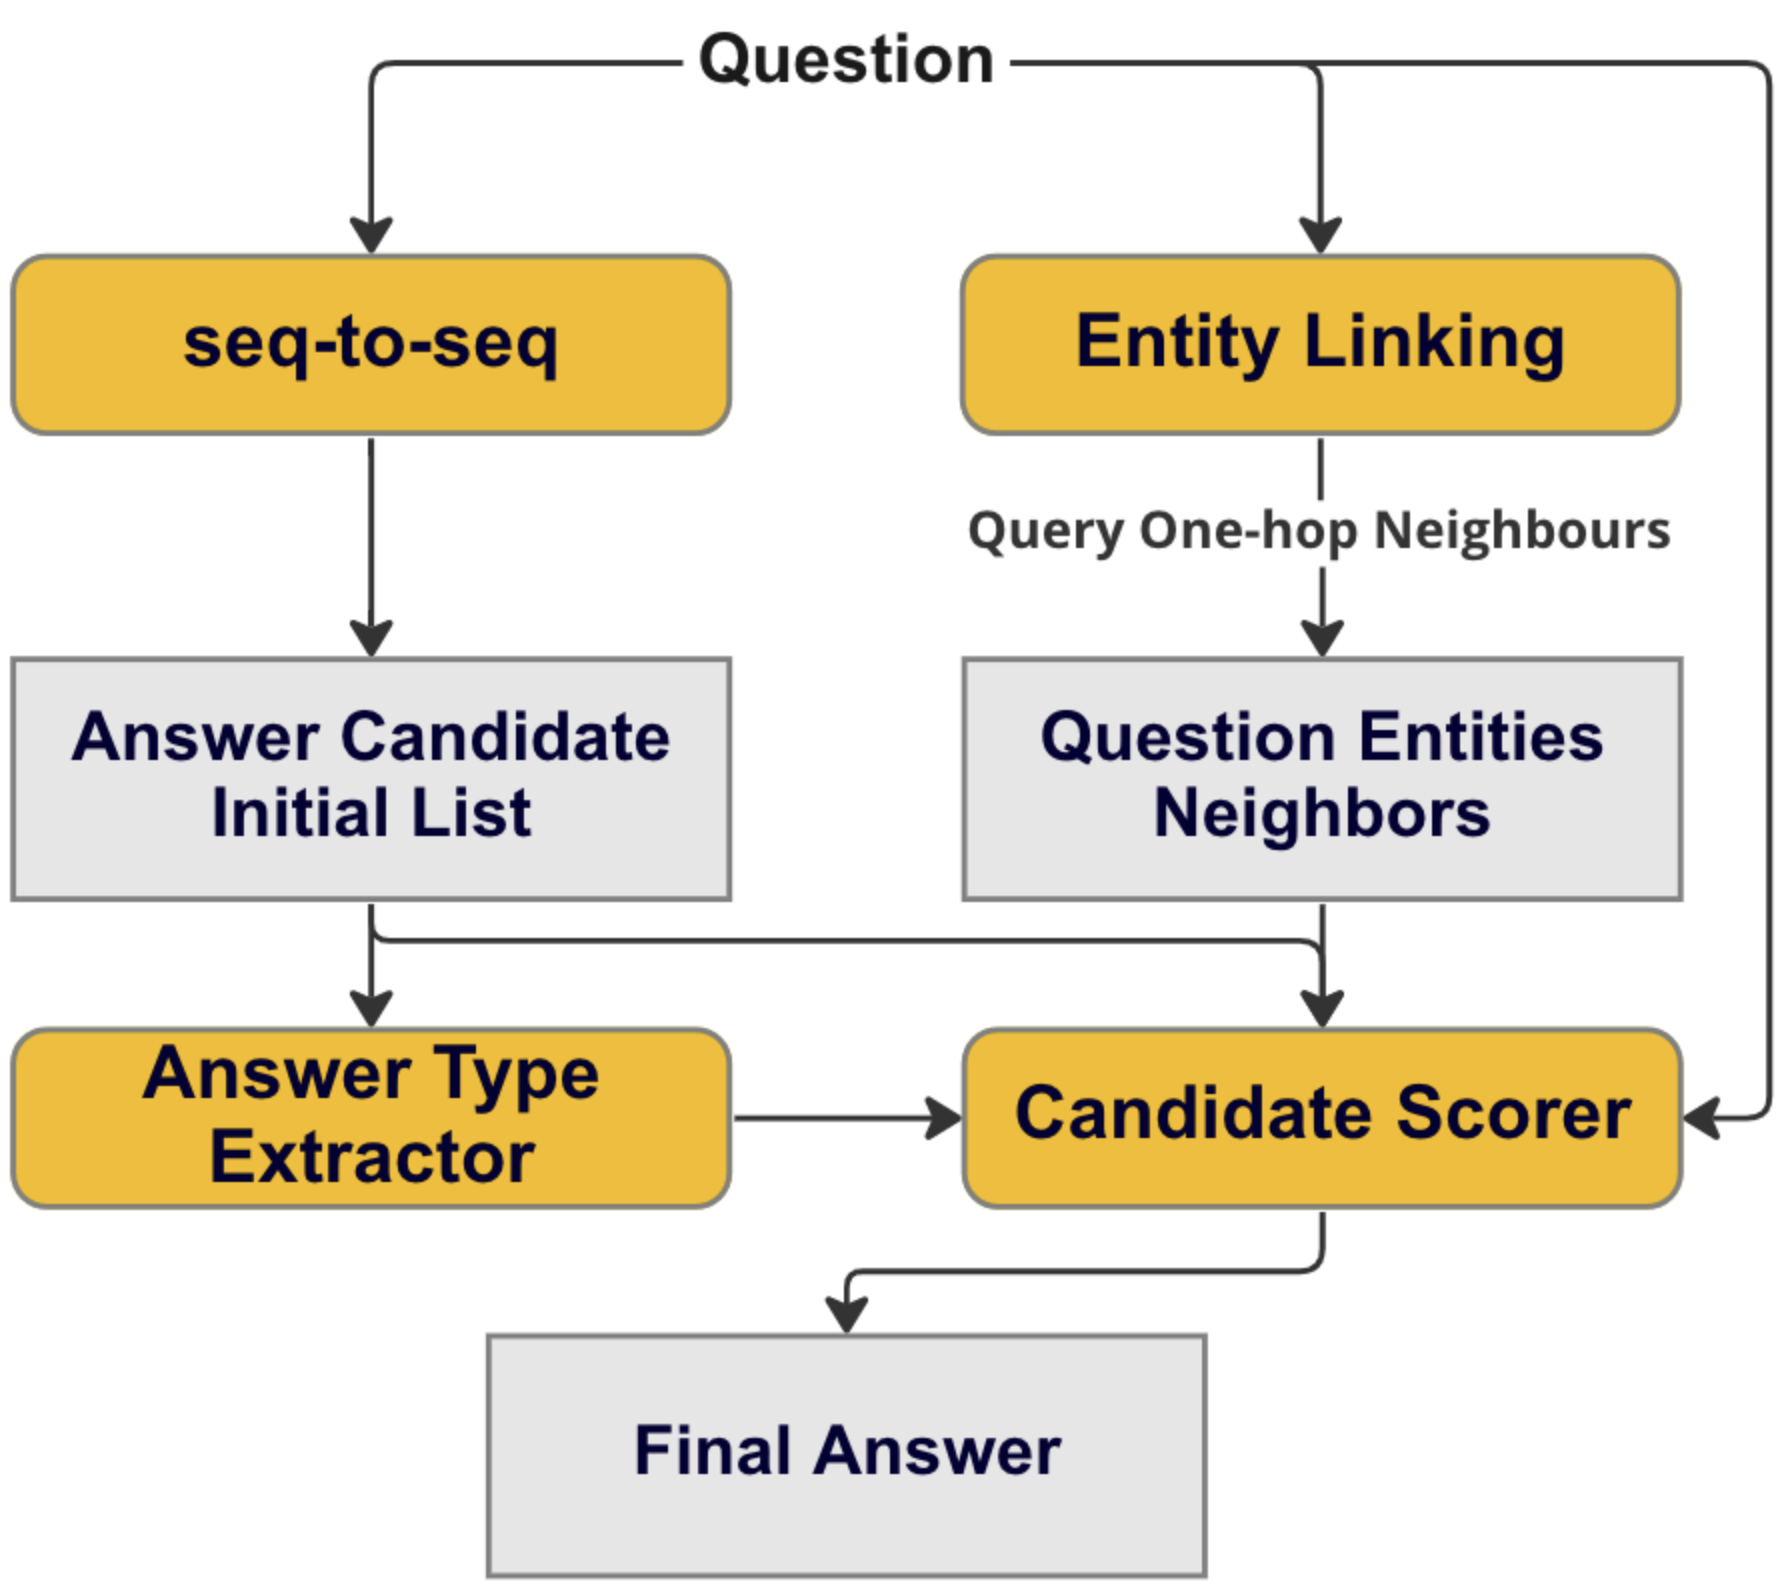
\includegraphics[width=0.85\textwidth]{act_selection/pipeline.png}
    \caption{ACT Selection Pipeline: (1) Put question to sequence to sequence language model to generate answer candidates, (2) Extract type from candidates, (3) Extract entities from the questions and query one-hop neighbors of the entities in the KG, (4) Filter candidates by type, (5) Select the best candidate.}
    \label{fig:act_selection:pipeline}
\end{figure}

\begin{figure}[h]
    \centering
    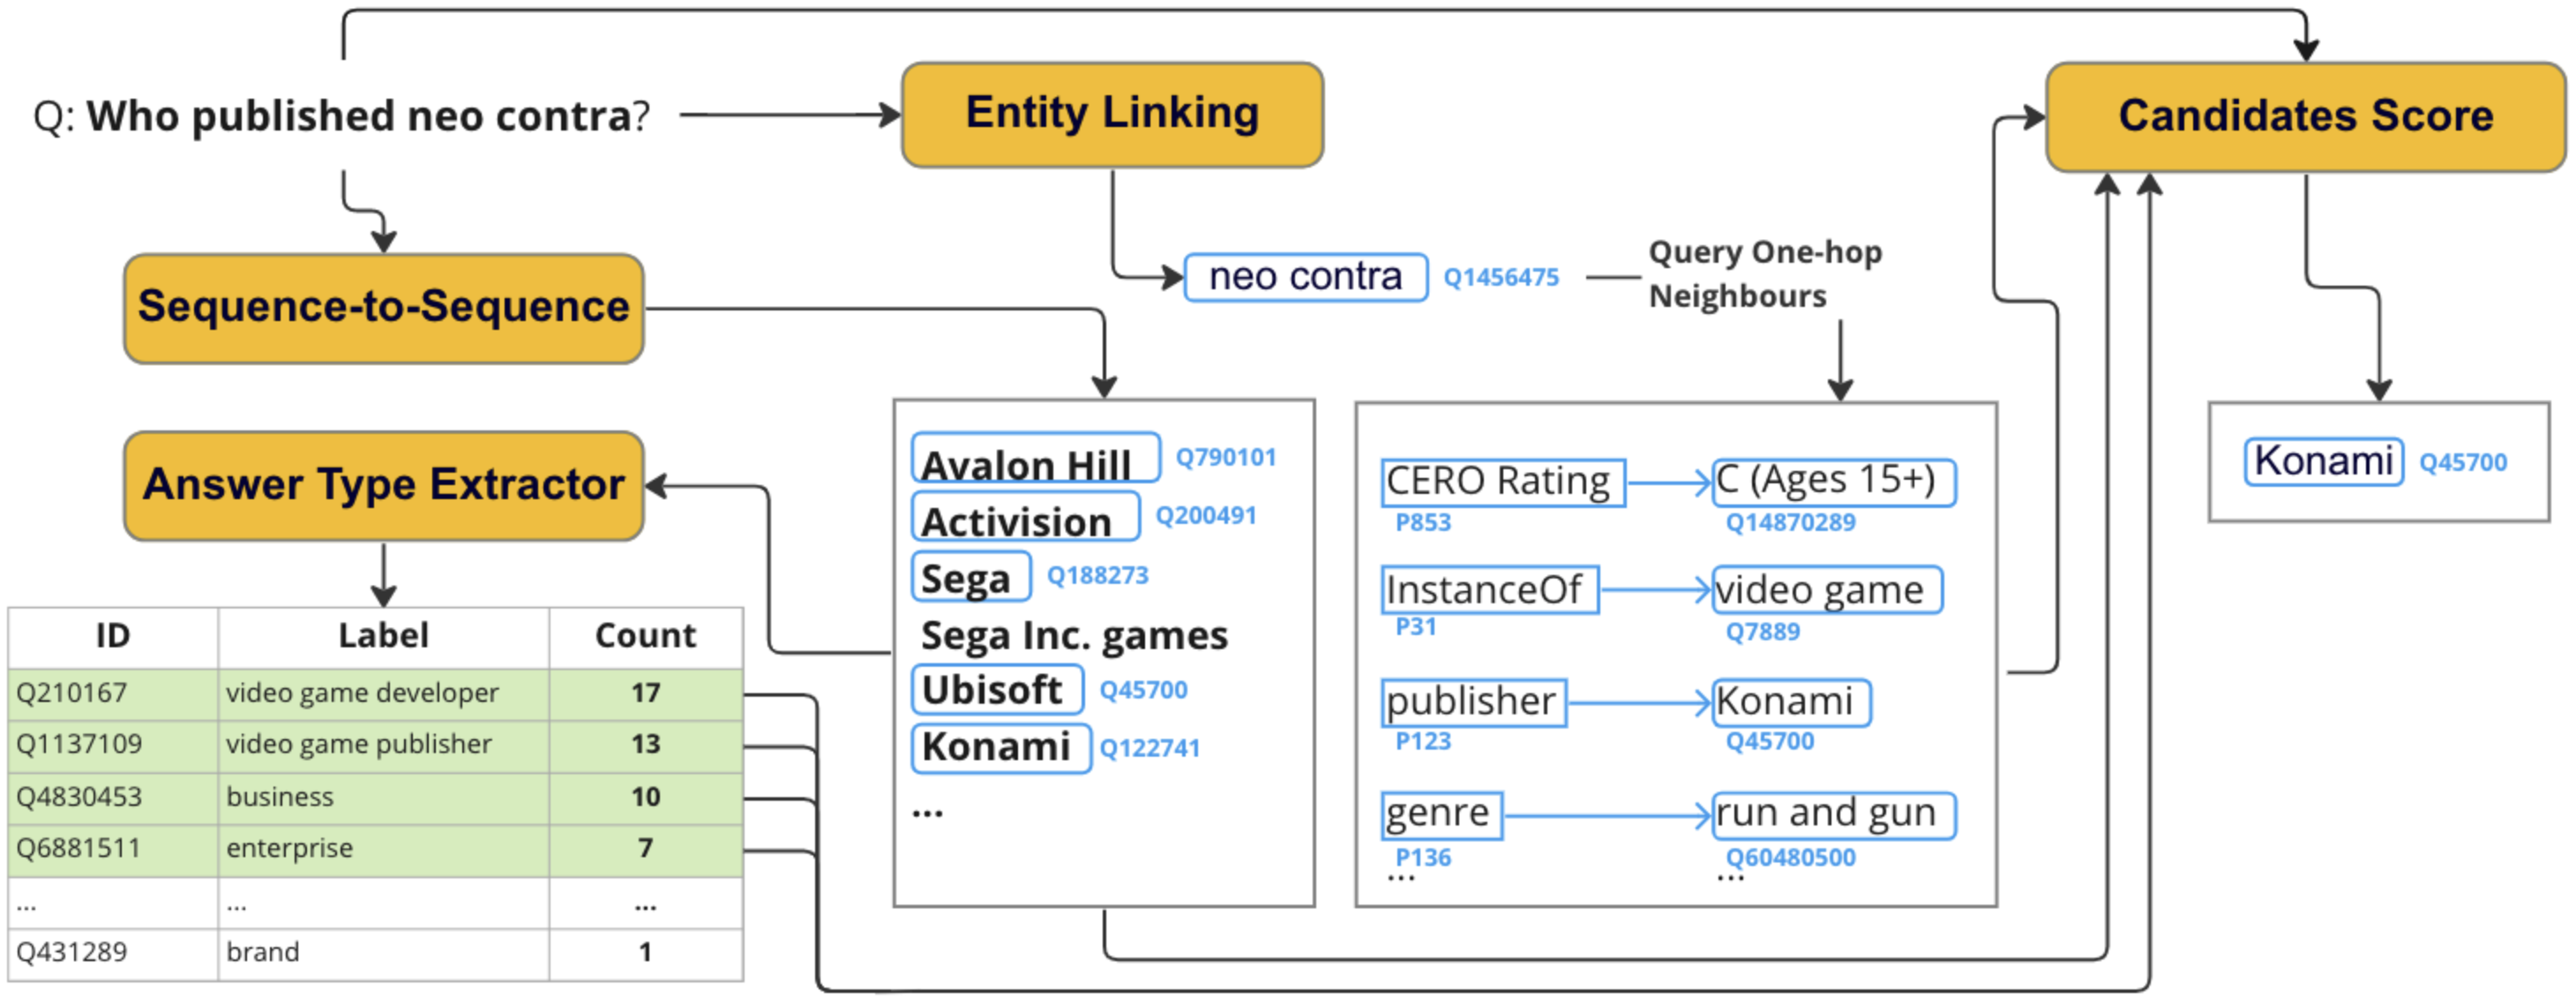
\includegraphics[width=0.95\textwidth]{act_selection/pipeline_example.png}
    \caption{The Answer Candidate Type (ACT) Selection pipeline for Knowledge Graph Question Answering (KGQA). The process combines a sequence-to-sequence model with knowledge graph-based entity linking and scoring to identify the correct answer, "Konami," as the publisher of "Neo Contra."}
    \label{fig:act_selection:pipeline_example}
\end{figure}

\subsection{Initial Answer Candidate List Generation} 
To increase the diversity of the generated results, we use Diverse Beam Search~\cite{DBLP:journals/corr/VijayakumarCSSL16-diverse-beam-search} to generate an initial list of answer candidates $C$. It often leads to a better exploration of the search space by ensuring that alternative answers are considered. It will discussed in more detail in Section~\ref{sec:methods_kg_path_fusion:expansion_of_generated_candidates}. We define the types of entities using the Wikidata property \texttt{instance\_of}~(P31). Note that an entity can be of multiple types. Finally, the initial list of answer candidates is used in the Answer Candidate Typing and the Candidate Scorer with the mined candidates. 

\subsection{Answer Candidate Typing} \label{act}
We rank all types by their frequency in the initial list of answer candidates. 
After that, we merge the top-$K$ most frequent types and similar types to the final list $T$.
Types similarity is calculated as cosine similarity between Sentence-BERT~\cite{reimers-2019-sentence-bert} embeddings of respective labels. The final types are defined as the ones where similarity is greater than a threshold.

A similar aggregation method using hypernyms (also known as ''is-a''  or ''instance-of'' relations) was used in the past to label clusters of words senses in distributional models~\cite{biemann2013text}: distributionally similar words share common hypernym and top common hypernyms are surprisingly good labels for sense clusters. The analogy in our method is that language models appear to produce a list of distributionally similar candidates.

\subsection{Entity Linking}
To enrich the list of candidates, we add all one-hop neighbors of the entities found in the question. For that, we use the fine-tuned spaCy Named Entity Recognition~(NER)\footnote{\url{https://spacy.io}.}

Based on a comprehensive review of state-of-the-art Named Entity Recognition (NER) systems \cite{vajjala-balasubramaniam-2022-really}, we evaluated the top three approaches: spaCy\footnote{\url{https://spacy.io}}, Stanza\footnote{\url{https://stanfordnlp.github.io/stanza/}}, and SparkNLP\footnote{\url{https://nlp.johnsnowlabs.com}}. Our analysis revealed that pre-trained NER models performed poorly on the Simple Question Wikidata (SQWD)~\cite{SQ_WD} dataset, with entity detection failure rates ranging from 64\% to 88\%. Among these systems, spaCy demonstrated the best performance, leading us to select its standard configuration\footnote{\url{https://spacy.io/usage/training/}} for further fine-tuning. The implementation of this pipeline required two critical pre-processing steps. First, we needed to identify the entity span to feed into the algorithm. This necessitated first extracting entity labels and their corresponding redirects, then locating these labels within the question text to determine spans. For entities without exact matches in the question, we employed fuzzy search techniques\footnote{\url{https://pypi.org/project/fuzzywuzzy/}}. Second, spaCy's training process requires entity type tags (e.g., PERSON for "Elon Musk", ORG for "Tesla" - following the BIO tagging scheme), which were not provided in the original datasets. We initially assigned the PERSON tag universally across all entities. Subsequent experiments with more precise entity type tagging did not yield significant improvements.
After extensive evaluation, we ultimately selected mGENRE \cite{decao2021multilingual} as our entity linking solution, which demonstrated superior performance compared to the NER-based approaches. mGENRE functions as an end-to-end entity linking system that eliminates the need for separate entity detection and disambiguation steps. Its multilingual autoregressive entity linking capabilities provided better accuracy and robustness across diverse question formulations in our experiments, making it a practical choice for our knowledge graph question answering pipeline.

\subsection{Candidates Scorer}
Finally, we calculate four scores for each entity from the answer candidate and rank them based on the weighted sum of the scores.
The scores are as follows:
% \begin{itemize}
    % \item
    \textbf{(1)~Type score} represents the size of the intersection between the set of types extracted from the answer candidates and the selected answer types. It is weighted by the number of selected answer types: $$S_\textrm{type}~=~\frac{|\textrm{Candidates' Types} \cap T|}{|T|}.$$

    % \item
\textbf{(2)~Forward one-hop neighbors score} $S_\textrm{neighbour}$ is  assigned 1 if the candidate is among the neighbors of the question entities, and 0 otherwise.

    % \item
\textbf{(3)~Text-to-Text answer candidate score} is determined by the rank of the candidate in the initial list $C$ generated by the Text-to-Text model divided by the size of the list: $$S_\textrm{t2t}~=~\frac{C.\textsc{}{index}(\textrm{Candidate})}{|C|}.$$

    % \item
\textbf{(4)~Question-Property Similarity score} $S_\textrm{property}$ measures the cosine similarity between the embeddings of the relevant property and the entire question. We employ Sentence-BERT~\cite{reimers-2019-sentence-bert} to encode the question, following a similar approach used for the Answer Candidate Type module.
% \end{itemize}
The four scores are calculated for each entity and then are combined to generate a final score that determines the entity's ranking. The answer with the highest weighted sum of scores in the candidate list is selected as the final answer:
%
$$S_\textrm{final} = S_\textrm{type} + S_\textrm{neighbour} + S_\textrm{t2t} + S_\textrm{property}.$$

% The weights for this sum can be estimated using logistic regression on a sample dataset in a future works.

% Text-to-Text models, despite occasionally providing incorrect answers, still yield answers of the correct type that can be utilized within the KGQA pipeline. This is demonstrated in the example depicted in Figure~\ref{fig:pipeline_example}.

% TODO: Добавить больше текста - заключение для метода 

% 3.2 Controllable Fusion using Knowledge Graph Paths
\section{Controllable Fusion using Knowledge Graph Paths}
\label{sec:methods_kg_path_fusion}

While constraining the answer type, as discussed in Section~\ref{sec:methods_type_selection}, provides a valuable signal for improving factuality, another powerful approach involves leveraging the explicit relational structure within the Knowledge Graph more directly. This section introduces methods based on the core idea of using KG subgraphs - a small part of the KG that contains the entities from the question, answer candidate generated by the LLM, and the shortest paths between them, drawing upon the work presented in \cite{DBLP:journals/corr/abs-2310-02166} and subsequent refinements focused on reranking 
{\color{red} TODO: add cite SWJ Reranking Answers of Large Language Models with Knowledge Graphs}.

The central motivation is to move beyond implicit knowledge within the LLM and provide explicit, verifiable evidence trails from the KG. Instead of solely relying on the LLM to generate a factually correct answer, we can use paths connecting entities mentioned in the question to potential answer entities within the KG as a strong indicator of factual consistency. This approach offers greater controllability and interpretability, as the KG path itself serves as evidence supporting a given answer.

The general pipeline for this fusion strategy, illustrated in Figure~\ref{fig:methods_kg_path_fusion:big_pipe}, involves several stages. First, relevant entities are identified within the input question. Second, candidate answers might be generated by an LLM, or potential answer entities are retrieved from the KG, focusing on entities connected to the question entities via relatively short paths. Crucially, features are extracted from these connecting paths (or the surrounding subgraph). These features capture information about the path structure and relations involved. Finally, these subgraph based features are used by a scoring or reranking model to evaluate the correctness of each candidate answer, ultimately selecting the answer best supported by the explicit structure of the Knowledge Graph. This section will detail the specific mechanisms developed for implementing this subgraph based fusion method.

\begin{figure}[htb]
    \centering
    \includegraphics[width=\columnwidth]{kg_path_fusion/new_paper_big_pipeline.pdf}
    \caption{The proposed method for reranking language model answers with KGs. The method includes subgraph extraction, features extraction, and various ranker approaches.}
    \label{fig:methods_kg_path_fusion:big_pipe}
\end{figure}
  
% In this section, we examine each component of the process in detail.
%  Firstly, we generate answer candidates using various LLMs and generate subgraphs, as discussed in Subsection~\ref{sec:subgraph_extract}. Next, in Subsection~\ref{sec:subgraph_features}, we will look at which attributes are used to rank responses.

\subsection{Answer Candidate Generation} \label{sec:methods_kg_path_fusion:expansion_of_generated_candidates}
As the subgraph extraction protocol requires answer candidates, we need a source of distinct answer candidates for each question, but most LLM approaches for QA, such as the one presented by \cite{DBLP:conf/coling/SenAS22-mintaka}, typically use \texttt{Greed Search} and evaluate the top-1 answer, it is important to note that the correct answer may not always be the top candidate. For example, the fine-tuned T5-XL-SSM~\cite{DBLP:conf/emnlp/RobertsRS20} model achieved higher Mean Reciprocal Rank (MRR) scores for our task, indicating that re-ranking could improve the top-1 results. 
However, even when using \texttt{Classical Beam Search}, the output is often minor variations of a single sequence, which may not generate enough unique answer candidates for the Question Answering task. Similar to the approach a little bit described in Section~\ref{sec:methods_type_selection}, we use Diverse Beam Search~\cite{DBLP:journals/corr/VijayakumarCSSL16-diverse-beam-search} to generate an initial list of answer candidates.

The formula~\ref{eq:methods_kg_path_fusion:diverse_beam_search} involves splitting the set of beams at time $t$ into $g$ disjointed subsets $Y_{[t]}^g$, and then selecting the candidate with the highest diversity penalty, which is calculated as the sum of a diversity penalty function $\Theta(y_{b,[t]}^g)$ over all candidates in the subset. Additionally, a dissimilarity term is included, which is calculated as the sum of a dissimilarity function $\Delta(y_{b,[t]}^g, Y_{[t]}^h)$ over all previous subsets $Y_{[t]}^h$ up to time $g-1$. The dissimilarity term is weighted by a parameter $\lambda_g$. This formula is used to optimize the selection of answer candidates in a computationally efficient manner.

\begin{equation}
    \begin{aligned}
        Y_{[t]}^g = \quad & \underset{y_1^{g}, \dots, y_{B\prime}^g \in Y_t^g} {\text{argmax}} \quad \underbrace{\sum_{b \in [B\prime]} \Theta(y_{b, [t]}^g)}_{\text{diversity penalty}} \\ 
        & + \underbrace{\sum_{h=1}^{g-1} \lambda_g \Delta(y_{b,[t]}^g, Y_{[t]}^h)}_{\text{dissimilarity term}},
    \end{aligned} 
    \label{eq:methods_kg_path_fusion:diverse_beam_search}
\end{equation}

% We apply {Diverse Beam Search} to the following LLMs: {T5-large-ssm}, {T5-XL-ssm}, {Mistral}, and {Mixtral} with $200$ beams, $20$ beam groups, and a $0.1$ diversity penalty. We extend our previous research~\cite{DBLP:conf/paclic/SalnikovLRNBMP23-originalpaper} by fine-tuning the proposed T5-like models and comparing them to more recent state-of-the-art models like Mistral and Mixtral, which should make our research more applicable to real-world use cases. T5-large-SSM and T5-XL-SSM were reported to be state-of-the-art both in the original Mintaka paper and our previous work, serving as a good baseline for comparison in this study.

% To finetune the T5-like models, we first train them on English questions for $10000$ steps, following the protocols outlined in the original Mintaka paper~\cite{DBLP:conf/coling/SenAS22-mintaka}. For the more state-of-the-art Mistral and Mixtral, we finetune with LoRA and train on English questions by generating the answer candidates with ``\textit{Answer as briefly as possible without additional information. [Question]}''. However, for the T5-like models, despite adhering to these protocols, we could not achieve the reported Hits@1 accuracy in the original paper. Despite this challenge, the main focus of the study is on the reranking aspect of the pipeline. Therefore, this paper's primary contribution is improving our fine-tuned models.

\subsection{Subgraph Extraction} \label{sec:subgraph_extract}
The main backbone of our approach is the procedure of subgraph extraction. We rely on the information conveyed in the relationships between question-answer pairs to improve the reranking of LLM generations. To further investigate how this relationship can improve performance, we employ a subgraph extraction algorithm that generates a KG's subgraph containing entities relevant to each question-answer pair and the shortest paths between them that contain relevant properties/relationships. 
% We extract various features that can be used for reranking in addition to the subgraphs. This section presents the subgraph extraction algorithm, the features derived from the subgraphs, and our reranking approaches.

\begin{figure}[htb]
    \centering
    \includegraphics[width=\columnwidth]{kg_path_fusion/ssp_to_sub.pdf}
    \caption{The proposed method for reranking language model answers with KGs. The method includes subgraph extraction, features extraction, and various ranker approaches.}
    \label{fig:methods_kg_path_fusion:subgraph_construction_example}
\end{figure}

For each question-answer candidate pair, the desired subgraph $G$ is mathematically defined as an induced subgraph of the Knowledge Graph. Thus, given our shortest paths from $e_i~\rightarrow~A$, where $e_i$ - entity extracted from question and $A$ - Answer. We can use the following Listing~\ref{alg:methods_kg_path_fusion:sub_extract} to extract $G$. Let us define $H$ as the set of all distinct nodes within our shortest paths $P_i$. We want to preserve all edges between the nodes within $H$. For all question-answer pairs, our objective is to retain the relationship between our question entities $E$ and answer candidate entity $A_i$. The process is schematically depicted at Figure~\ref{fig:methods_kg_path_fusion:subgraph_construction_example}.

\begin{ListingEnv}[p]
    \centering % Center the listing if desired
    \caption{Subgraph Extraction Algorithm} 
    \label{alg:methods_kg_path_fusion:sub_extract} 
    \begin{lstlisting}[basicstyle=\fontsize{10pt}{12pt}\selectfont\ttfamily] % Smaller font for code Require: entities, candidate

paths = []
For entity in entities:
    shortest_paths = get_shortest_path(entity, candidate)
    paths.extend(shortest_paths)

H = set of unique nodes in paths

G = new Graph()
Add nodes from H to G

For unique_node in H:
    unique_node_neighbors = get_neighbors(unique_node)
    For neighbor_node in unique_node_neighbors:
        If neighbor_node in H:
            Add edge (unique_node, neighbor_node) to G

Return G
    \end{lstlisting}
\end{ListingEnv}


\subsection{Features based on Extracted Subgraphs} \label{sec:methods_kg_path_fusion:subgraph_features}
After extracting subgraphs for all answer candidates of our LMs, we use all possible useful features for reranking. Referring to our previous study, we mainly focused on a simple text representation of the extracted subgraphs to rank our answer candidates. Thus, in this study, we propose extracting as many useful features as possible and analyzing each feature's importance in this reranking problem. We have divided the features into the following main categories: graph, text, and Graph2Text sequence features. 

\subsubsection{Graph Features} \label{sec:methods_kg_path_fusion:graph_features}
With our extracted subgraphs and their corresponding answer candidate, we seek to use the relationship from the subgraphs to classify the correct answer candidate. As the first simple baseline, we utilize graph features consisting of simple numerical subgraph statistics. We hypothesize that subgraphs with the correct answer will be less ``complex'' than subgraphs with the incorrect answer candidate. Therefore, we would want the graph features to convey the complexity of the respective subgraph. With a clear objective in mind, we experiment with the following graph features:  

\begin{itemize}
    \item \textbf{Number of nodes and edges}: basic statistics of the nodes and edges of graph $G$.
    \item \textbf{Number of cycles}: a cycle of graph $G$ is a non-empty path that starts from a given node and ends at the same node. 
    \item \textbf{Number of bridges}: a bridge of graph $G$ is an edge, where its deletion increases the number of connection components. 
    \item \textbf{Average shortest path}: the average of each shortest path between the question entity and the answer entity. 
    \item \textbf{Density}: measurement of the density of a graph, where the number of edges in a dense graph is close to the maximal number of edges (each pair of nodes is connected by an edge). The density $d$ for the graph $G$ is formulated as $d = \frac{m}{n(n-1)}$, where $n$ is the number of nodes and $m$ is the number of edges in $G$.
   \item \textbf{Katz centrality}~\cite{katz1953new}: measurement of the importance (or ``centrality'' - how ``central'' a node is in the graph) of a specific node $i$ in a graph $G$. The Katz centrality for node $i$ of graph $G$ is formulated as $x_i = \alpha \sum_{j} A_{ij} x_j + \beta$, where $A$ is the adjacency matrix of graph $G$ with eigenvalues $\lambda$, $\beta$ is the parameter that controls the initial centrality, and $\alpha < \frac{1}{\lambda_{\max}}$. 
    \item \textbf{PageRank}~\cite{page1999pagerank}: a popular algorithm used by Google to rank web pages in the search query by counting the number and quality of links to a page to determine an estimate of its importance. In graph theory, the ``web pages'' and ``links'' are synonymous with nodes and edges. 
\end{itemize}

\noindent We hypothesize that these features may provide ranker models with insights into the complexity of the respective subgraphs.


\subsubsection{Text Features} \label{sec:methods_kg_path_fusion:text_features} The ablation study showcased the importance of including the question within the text representation of the subgraph. Therefore, besides the simple graph features, we want to emphasize each question/answer pair without using extracted subgraphs. Thus, the text features represent the concatenation between the question and answer, separated by a semicolon --- ``\texttt{;}''. To use this simple concatenation for all ranker approaches, we encode the string using the MPNet\footnote{\url{https://huggingface.co/sentence-transformers/all-mpnet-base-v2}} embedding model~\cite{DBLP:conf/nips/Song0QLL20}.


\subsubsection{Graph2Text Sequence Features} \label{sec:methods_kg_path_fusion:g2t_seq} 
Given the vast amount of data contained in Knowledge Graphs, it is essential to convert this information into natural language to facilitate understanding and accessibility. Converting a graph into text, known as KG-to-text or Graph2Text, has demonstrated notable success in various applications~\cite{DBLP:journals/corr/abs-2309-11206}. Therefore, when generating text from a Knowledge Graph, it is crucial to analyze the underlying graph structure carefully to ensure accurate translation.

Without an obvious way of incorporating the question within the subgraphs, relying purely on the subgraphs to rerank is ineffective~\cite{DBLP:conf/paclic/SalnikovLRNBMP23-originalpaper}. Therefore, we address this issue by further exploration of different KG-to-text methods. The main objective is experimenting with various techniques to represent the extracted subgraphs more explicitly. For this type of textual feature, we researched and developed three methods for representing subgraphs as a text, including \textbf{Graph2Text Deterministic,  Graph2Text T5, and  Graph2Text GAP}.

Firstly, we employ the \textbf{Graph2Text Deterministic} approach, the most straightforward text linearization approach. In simple terms, the subgraphs are unraveled by their matrix representation. Firstly, to linearize, we convert the subgraph into its binary adjacency matrix. Let us call it matrix $A$. 
Given $n$ nodes in the subgraph, the resulting matrix's dimension will be $n \times n$. The matrix's element $[i, j]$ represents the existence of an edge between a node with index $i$ and a node with index $j$. Then, we replace the edges in the matrix with the edge label and call it $A'$. 
Adjacency matrices are typically implemented with graphs with numeric weights. The weights were string representing the relationship between our nodes. Thus, we represented the existence of an edge with $1$, then replaced in the edge with the string relationship.
%Let us call this adjacency matrix with edge information . 
Lastly, we unravel $A'$ row by row to produce our final sequence and add the triple (node\_from, edge, node\_to) to our final sequence. Listing~\ref{alg:methods_kg_path_fusion:sub2seq} summarizes the aforementioned steps. 

\begin{ListingEnv}[p]
    \centering % Center the listing if desired
    \caption{Subgraphs to Sequence - Graph2Text Deterministic} 
    \label{alg:methods_kg_path_fusion:sub2seq} 
    \begin{lstlisting}[basicstyle=\fontsize{10pt}{12pt}\selectfont\ttfamily] % Smaller font for code

Require: Subgraph G
Ensure: Text representation of subgraph Seq

adj_matrix = get_adjacency_matrix(G)
Seq = ""
# Assuming adj_matrix is n x n, where n is number of nodes
# and indices correspond to node IDs
For i in range(number_of_nodes(G)): 
    For j in range(number_of_nodes(G)):
        # Assuming 0 indicates no edge, non-zero indicates an edge
        If adj_matrix[i][j] != 0: 
            # Assuming G allows lookup by index i, j
            node_i_label = get_node_label(G, i) 
            node_j_label = get_node_label(G, j)
            # Get edge info (label/type) between node i and j
            edge_info = get_edge_info(G, i, j) 
            # Append triple to sequence string, separated by e.g., semicolon
            Seq += node_i_label + " " + edge_info + " " + node_j_label + "; " 
Return Seq
    \end{lstlisting}
\end{ListingEnv}

For the remaining two text linearization approaches, \textbf{Graph2Text T5} and \textbf{Graph2Text GAP}, we employ more complex neural-based models trained on the WebNLG~2.0 dataset~\cite{DBLP:conf/acl/GardentSNP17}. This dataset consists of instances, where each includes a Knowledge Graph from DBpedia~\cite{DBLP:conf/semweb/AuerBKLCI07} and a target text comprising one or more sentences that describe the graph. The test set is divided into partitions of seen (DBpedia categories present in the training set) and unseen (DBpedia categories not present in the training set). The statistics of this hand-crafted and human-verified dataset are described in detail in Table~\ref{tab:methods_kg_path_fusion:webnlg_label}. 

\begin{table}
    \centering
    \caption{Statistics of the WebNLG 2.0 parallel knowledge graph-to-text dataset.}
    
    \begin{subtable}[t]{0.48\textwidth}
    \centering
    \begin{tabular}{lr}
        \toprule
        \textbf{Entities} & 2,730 \\
        \textbf{Relations} & 354 \\
        \textbf{Triples} & 81,927 \\
        \bottomrule
    \end{tabular}
    \caption{Knowledge Graph statistics. Total number of KG components, number of tokens in the narratives.}
    \label{tab:kg_stats}
    \end{subtable}
    \hfill
    \begin{subtable}[t]{0.48\textwidth}
    \centering
    \begin{tabular}{lr}
        \toprule
        \textbf{Total} & 623,902 \\
        \textbf{Unique} & 8,075 \\
        \textbf{Entity} & 60\% \\
        \bottomrule
    \end{tabular}
    \caption{Texts statistics. The percentage of text entities represents the portion of the text that includes entity labels.}
    \label{tab:methods_kg_path_fusion:webnlg_label}
    \end{subtable}
\end{table}

The idea behind the \textbf{Graph2Text T5} approach is to extract informative and useful features from KGs using pre-trained text-to-text LMs. With the impressive capabilities of pretrained LMs in the text-to-text generation task, we seek to replicate such results in the graph-to-text scope. Our idea is built upon the analogous algorithm discussed in~\cite{DBLP:journals/corr/abs-2007-08426}. The authors tackle the graph-to-text generation task in this work with two popular text-to-text pre-trained LMs, BART and T5. These models have an encoder-decoder architecture, which makes them well-suited for conditional text generation tasks. To adapt these models for the graph-to-text task, the authors continue pre-training BART and T5 using the following approaches:

\begin{enumerate}
    \item Language Model Adaptation (LMA): the models are trained on reference texts that describe graphs, following the BART and T5 pre-training strategies.
    \item Supervised Task Adaptation (STA): the models are trained on pairs of graphs and their corresponding texts collected from the same or a similar domain as the target task --- graph-to-text in this case. 
\end{enumerate}

Building on the STA approach via T5 and WebNLG~2.0, we obtain graph-to-text sequences by first converting the graph into a sequence of tokens through linearization. We use the string ``convert the [graph] to [text]:'' to acquire this linearised sequence. This output sequence is then fed into the input sequence for the T5 model tuned on WebNLG~2.0. 
% For tuning Graph2Text T5 approach, we use the following hyperparameters: \textit{learning rate}: $1e^{-3}$, \textit{batch size}: 4, \textit{gradient accumulation steps}: 32, and \textit{Adam optimizer}. 

The \textbf{Graph2Text GAP} approach is based on the current state-of-the-art graph-to-text task, GAP, built on BART~\cite{DBLP:conf/coling/ColasAW22-GAP}. 
The main idea of GAP is a fully graph-aware encoding combined with the coverage of pre-trained LMs. The GAP KG-to-text framework fuses graph-aware elements into existing pre-trained LMs, capturing the advantages brought forth by both model types. The architecture of this solution consists of two main components:

\begin{enumerate}
\item \textbf{Global Attention}: to capture the graph's global semantic information, the graph’s components are first encoded using an LM. This allows the model to leverage the lexical coverage of pre-trained LMs.
\item \textbf{Graph-aware Attention}: to attend to and update the representations of entities, relations, or both, a topological-aware graph attention mechanism was introduced, which includes entity and relation type encoding.
\end{enumerate}

Applying the work of GAP, we first linearize the input graph into a text string by creating a sequence of all triples in the KG, interleaved with tokens that separate each triple and the triple's components (head, relation, and tail). Then, we use a transformer encoder to obtain vector representations. The first module in each transformer layer acts as a Global Attention and captures the semantic relationships between all tokens. Moreover, we use a Graph-aware Attention module to capture the sparse nature of adjustment in a graph and apply it to entity and relation vectors from word vectors. By proposing this flexible framework, where graph-aware components can be interchanged, the current architecture aims to generate coherent and representative text descriptions of the KG. Like the Graph2Text T5 approach, we pretrain the model on the WebNLG~2.0 dataset and get the final predictions through the fine-tuned model. 
% For finetuning the Graph2text GAP approach, we use the following hyperparameters: \textit{learning rate}: $2e^{-5}$, \textit{batch size}: 16; \textit{beam size}: 5, \textit{Adam Optimizer}, 50 \textit{nodes}, and 60 \textit{relations}.


% In this research, we introduce the more complex neural-based graph-to-text approach to explore further the reranking capabilities of the textual representation of our extracted subgraphs. The initial rudimentary text linearization approach has already achieved state-of-the-art Hits@1. We look for a more complete case study on reranking the text linearization with these two neural-based linearization approaches. To further digest the two methods, a comparison between the Graph2Text T5 and Graph2Text GAP sequences can be seen in the table ~\ref{tab:example_of_predictions_label}. Additionally, for better visualization, we implement a web application that automatically applies the T5 and GAP approaches to the desired subgraph, discussed in detail in Section ~\ref{sec:webapp}.
 

% \input{tabs/graph2text_examples}
% All three variation of Graph2Text Sequence features are further encoded with MPNet embedding model~\cite{DBLP:conf/nips/Song0QLL20}, discussed more in \ref{appx:detailed_results}. Moreover, motivated by our previous research, we employ context and highlight these Graph2Text sequences, discussed further in \ref{hl_context}.


% 3.3 Experimental Design and Baselines
\section{Experimental Design and Baselines}
\label{sec:methods_experimental_design}
% Comment: Describe the experimental setup used to evaluate the methods in 3.1 and 3.2. 
% Specify the datasets used (you might briefly introduce the motivation for ShortPathQA 
% here, leading into the next chapter), the evaluation metrics focused on factuality 
% and accuracy, and the baseline models (including perhaps zero-shot/few-shot LLMs, 
% and simpler KGQA systems).


% 3.4 Results and Analysis: Demonstrating Factuality Improvements
\section{Results and Analysis: Demonstrating Factuality Improvements}
\label{sec:methods_results}
% Comment: Present the quantitative results comparing your methods against baselines. 
% Crucially, analyze *why* your methods work, using examples and error analysis to 
% show how KG fusion mitigates specific failure modes of standalone LLMs (e.g., 
% hallucinations, factual errors). Discuss the trade-offs of each method.          % Chapter 3: Methods (Previously foundations, now incorporates type selection and reranking/path fusion)
\chapter{Core Method II: Direct Question Answering using Knowledge Graph Paths (ShortPathQA)}
\label{ch:shortpathqa}

\section{Introduction}
\label{sec:shortpath:intro}
% TODO: Motivate direct KG-QA as an alternative to LLM generation/reranking.

\section{The ShortPathQA Approach}
\label{sec:shortpath:method}
% TODO: Describe the methodology from the NLDB paper.

\section{Dataset Creation}
\label{sec:shortpath:dataset}
% TODO: Detail your work on creating the ShortPathQA dataset.

\section{Experimental Setup}
\label{sec:shortpath:setup}
% TODO: Describe the experiments conducted (baselines, metrics).

\section{Results and Analysis}
\label{sec:shortpath:results}
% TODO: Present the full experimental evaluation results.
% TODO: Compare performance characteristics with other potential approaches.

\section{Discussion}
\label{sec:shortpath:discussion}
% TODO: Discuss the strengths (e.g., precision) and weaknesses (e.g., coverage, flexibility) of this method.

\section{Chapter Summary}
\label{sec:shortpath:summary}
% TODO: Summarize the main contributions and findings regarding ShortPathQA.  % Chapter 4: ShortPathQA Benchmark (Previously chapter_5)
\chapter{ShortPathQA: A Benchmark for Knowledge Graph Question Answering}
\label{chap:shortpathqa}

\section{Introduction}
\label{sec:shortpath:intro}
Building on the methods for answer candidate generation (Chapter~\ref{chap:candidate_generation}) and controllable fusion using knowledge graph paths (Chapter~\ref{chap:controllable_fusion}), this chapter introduces ShortPathQA, a novel benchmark for directly evaluating knowledge graph question answering capabilities. While the previous chapters focused on techniques to enhance LLM-generated answers with knowledge graphs, ShortPathQA explores a complementary approach that focuses on extracting precise answers directly from knowledge graph paths.

\section{The ShortPathQA Approach}
\label{sec:shortpath:method}
% TODO: Describe the methodology from the NLDB paper.

\section{Dataset Creation}
\label{sec:shortpath:dataset}
% TODO: Detail your work on creating the ShortPathQA dataset.

\section{Experimental Setup}
\label{sec:shortpath:setup}
% TODO: Describe the experiments conducted (baselines, metrics).

\section{Results and Analysis}
\label{sec:shortpath:results}
% TODO: Present the full experimental evaluation results.
% TODO: Compare performance characteristics with other potential approaches.

\section{Discussion}
\label{sec:shortpath:discussion}
% TODO: Discuss the strengths (e.g., precision) and weaknesses (e.g., coverage, flexibility) of this method.

\section{Chapter Summary}
\label{sec:shortpath:summary}
% TODO: Summarize the main contributions and findings regarding ShortPathQA.       % Chapter 5: System Demos (Previously chapter_8)
\chapter{On the Limits of Internalizing Knowledge: Insights from LoRA}
\label{chap:lora_limits}

% Comment: This chapter incorporates the findings from "How Much Knowledge Can You 
% Pack...", positioning it as an exploration complementary to the main KG fusion 
% theme.

% 6.1 Knowledge Integration Strategies: External vs. Internal
\section{Knowledge Integration Strategies: External vs. Internal}
\label{sec:lora_external_vs_internal}
% Comment: Revisit the idea of different ways to provide knowledge to LLMs. Contrast 
% the *external* approach (using KGs, as explored in Chapters 3-5) with *internal* 
% approaches like fine-tuning or parameter modification using methods like LoRA.


% 6.2 Investigating Knowledge Capacity in LoRA Adapters
\section{Investigating Knowledge Capacity in LoRA Adapters}
\label{sec:lora_capacity_investigation}
% Comment: Describe the study from "How Much Knowledge Can You Pack...". Explain the 
% methodology for "packing" knowledge into LoRA adapters and for measuring the 
% trade-off between acquired knowledge and the preservation of the base LLM's general 
% abilities.


% 6.3 Findings and Implications for KG-LLM Approaches
\section{Findings and Implications for KG-LLM Approaches}
\label{sec:lora_implications}
% Comment: Present the key results regarding the capacity limits of LoRA for storing 
% knowledge. Discuss the implications: Do these findings suggest inherent limitations 
% to solely relying on internalizing knowledge within LLM parameters, especially for 
% vast, dynamic factual information? Argue how these results might strengthen the case 
% for hybrid approaches that leverage external, structured knowledge sources like KGs 
% for robust factuality. 

\chapter{System Demonstrations and Implementation}
\label{chap:system_demos}

\section{Introduction}
\label{sec:demo:intro}
This chapter showcases the practical implementations of the methods discussed in earlier chapters. Moving from theoretical foundations to real-world applications, we present system demonstrations that illustrate how the fusion of Large Language Models (LLMs) and Knowledge Graphs (KGs) can be deployed to address factoid question answering tasks. These implementations serve not only as proof-of-concept for our methodological contributions but also as usable tools for researchers and potential end-users in the field.

\section{System for Answering Simple Questions}
\label{sec:demo:simple_qa}
% TODO: Describe the demo system from the ACL Demo paper.
% TODO: Explain its architecture and functionality.
% TODO: Connect it to the core methods discussed earlier.
% TODO: Mention your role in its development.

\section{Web Application for Knowledge Graph Path Visualization}
\label{sec:demo:kg_path_viz}
% TODO: Describe the web application for visualizing knowledge graph paths.
% TODO: Explain how it helps users understand the paths connecting entities.
% TODO: Discuss implementation details and technologies used.

\section{Reranking Demonstration Tool}
\label{sec:demo:reranking}
% TODO: Describe the demonstration tool for reranking answers.
% TODO: Explain how it incorporates the controllable fusion techniques.
% TODO: Showcase example usage and interface design.

\section{Integration with External Systems}
\label{sec:demo:integration}
% TODO: Discuss how these components can be integrated with other systems.
% TODO: Address API design, modularity, and extensibility.

\section{Chapter Summary}
\label{sec:demo:summary}
% TODO: Summarize the key takeaways from the demonstrations.        % Chapter 6: LoRA Limits (New chapter)
% \chapter{Application: Enhancing Comparative Question Answering with LLMs}
\label{ch:comparative_qa}

\section{Introduction}
\label{sec:compqa:intro}
% TODO: Introduce Comparative QA and the CAM 2.0 system.

\section{The CAM 2.0 System Architecture}
\label{sec:compqa:cam2_arch}
% TODO: Describe the overall architecture of CAM 2.0.

\section{LLM Integration and Fine-tuning}
\label{sec:compqa:llm_integration}
% TODO: Detail your contributions: LLM selection (Llama, Vicuna), fine-tuning process, integration challenges.

\section{Experimental Setup}
\label{sec:compqa:setup}
% TODO: Describe datasets, baselines, and evaluation metrics used for CAM 2.0.

\section{Results and Analysis}
\label{sec:compqa:results}
% TODO: Present the performance results, focusing on the impact of the LLM components you implemented.

\section{Discussion}
\label{sec:compqa:discussion}
% TODO: Discuss the effectiveness of LLMs in this complex QA task. Potential connections to KG methods.

\section{Chapter Summary}
\label{sec:compqa:summary}
% TODO: Summarize the findings regarding LLMs in comparative QA.  % Deleted - content integrated elsewhere
% \chapter{Integrated Evaluation and Comparative Analysis}
\label{ch:evaluation}

\section{Introduction}
\label{sec:evaluation:intro}
% TODO: Outline the goals of the integrated evaluation.

\section{Evaluation Framework}
\label{sec:evaluation:framework}
% TODO: Describe the benchmarks, metrics, and setup for comparison.

\section{Comparative Analysis: Core QA Methods}
\label{sec:evaluation:core_methods}
% TODO: Compare Reranking vs. ShortPathQA vs. Type Selection. Analyze trade-offs.

\section{Evaluation: LLMs in Comparative QA}
\label{sec:evaluation:comparative_qa}
% TODO: Present evaluation results for the LLM components in CAM 2.0.

\section{Overall Discussion}
\label{sec:evaluation:discussion}
% TODO: Synthesize the evaluation findings across all methods.

\section{Chapter Summary}
\label{sec:evaluation:summary}
% TODO: Summarize the main comparative insights.    % Deleted - content integrated elsewhere

% Note: chapter_3_subsection_type_selection.tex and chapter_3_subsection_kg_path_fusion.tex
% should be \input{}'ed inside chapter_3_methods.tex where appropriate.

\chapter{Conclusion and Future Work}
\label{chap:conclusion}

% 7.1 Synthesis of Contributions
\section{Synthesis of Contributions}
\label{sec:conclusion_synthesis}
% Comment: Provide a comprehensive summary of the thesis's achievements. Reiterate the 
% novel methods for KG-LLM fusion, the ShortPathQA benchmark contribution, system 
% demonstrations, and insights from related studies (LoRA). Emphasize the overall 
% narrative: identifying the LLM factuality problem and providing KG-based solutions.


% 7.2 Revisiting Research Questions
\section{Revisiting Research Questions}
\label{sec:conclusion_revisiting_rqs}
% Comment: Directly address the research questions posed in Chapter 1, providing 
% concise answers based on the evidence presented throughout the thesis.


% 7.3 Limitations of the Presented Work
\section{Limitations of the Presented Work}
\label{sec:conclusion_limitations}
% Comment: Honestly discuss the limitations of your research. This might include the 
% scope (e.g., focus on factoid QA), the specific KGs or LLMs used, scalability 
% challenges of the proposed methods, or aspects not fully explored.


% 7.4 Future Research Directions
\section{Future Research Directions}
\label{sec:conclusion_future_work}
% Comment: Propose concrete directions for future work building upon your thesis. 
% Examples: exploring more complex reasoning tasks, applying methods to different 
% domains or languages, integrating dynamic/temporal KGs, improving the efficiency 
% and scalability of fusion methods, developing more sophisticated control mechanisms, 
% investigating user interaction with KG-aware LLMs.       % Chapter 7: Conclusion (New chapter, replaces old conclusions.tex)
% \include{Dissertation/conclusions}      % Old conclusions include - replaced by chapter_7_conclusion

% \printnomenclature[3.5cm] % Значение ширины столбца с обозначениями стоит подбирать вручную


\addcontentsline{toc}{chapter}{List of symbols and abbreviations}
\chapter*{List of symbols and abbreviations}

\begin{tabularx}{0.9\textwidth}{lX}
    $I$ & Identity matrix \\
    $\mathcal{N}(\mu, \Sigma)$ & Gaussian distribution with mean vector $\mu$ and covariance matrix $\Sigma$\\
    $1\left[A\right]$ & Indicator of the event $A$ \\
    $PR(p_i)$ & PageRank of Graph $G$ node $p_i$ \\
\end{tabularx}        % List of Acronyms
% \include{Dissertation/dictionary}      % Dictionary of Terms (Optional)
\clearpage                                  % В том числе гарантирует, что список литературы в оглавлении будет с правильным номером страницы
%\hypersetup{ urlcolor=black }               % Ссылки делаем чёрными
%\providecommand*{\BibDash}{}                % В стилях ugost2008 отключаем использование тире как разделителя
\urlstyle{rm}                               % ссылки URL обычным шрифтом
\ifdefmacro{\microtypesetup}{\microtypesetup{protrusion=false}}{} % не рекомендуется применять пакет микротипографики к автоматически генерируемому списку литературы
% \printbibliography                           % Подключаем Bib-базы: все статьи единым списком
% Режим с подсписками
% \insertbiblioexternal                      % Подключаем Bib-базы: статьи, не являющиеся статьями автора по теме диссертации
% Для вывода выберите и расскомментируйте одно из двух
% \insertbiblioauthor                        % Подключаем Bib-базы: работы автора единым списком 
%\insertbiblioauthorgrouped                 % Подключаем Bib-базы: работы автора сгруппированные (ВАК, WoS, Scopus и т.д.)


\insertbiblioauthor
\insertbiblioexternal

\ifdefmacro{\microtypesetup}{\microtypesetup{protrusion=true}}{}
\urlstyle{tt}                               % возвращаем установки шрифта ссылок URL
%\hypersetup{ urlcolor={urlcolor} }          % Восстанавливаем цвет ссылок
      % Bibliography
\include{Dissertation/lists}           % List of Tables and Figures

\setcounter{totalchapter}{\value{chapter}} % Count chapters

%%% Appendices Setup
\appendix
% Оформление заголовков приложений ближе к ГОСТ:
\setlength{\midchapskip}{20pt}
\renewcommand*{\afterchapternum}{\par\nobreak\vskip \midchapskip}

\ifnumequal{\value{englishthesis}}{0}{
    \renewcommand\thechapter{\Asbuk{chapter}} % Чтобы приложения русскими буквами нумеровались
}{}

% \include{Dissertation/appendix}        % Приложения

\setcounter{totalappendix}{\value{chapter}} % Подсчёт количества приложений

\end{document}
